% Options for packages loaded elsewhere
\PassOptionsToPackage{unicode}{hyperref}
\PassOptionsToPackage{hyphens}{url}
%
\documentclass[
]{article}
\usepackage{amsmath,amssymb}
\usepackage{iftex}
\ifPDFTeX
  \usepackage[T1]{fontenc}
  \usepackage[utf8]{inputenc}
  \usepackage{textcomp} % provide euro and other symbols
\else % if luatex or xetex
  \usepackage{unicode-math} % this also loads fontspec
  \defaultfontfeatures{Scale=MatchLowercase}
  \defaultfontfeatures[\rmfamily]{Ligatures=TeX,Scale=1}
\fi
\usepackage{lmodern}
\ifPDFTeX\else
  % xetex/luatex font selection
\fi
% Use upquote if available, for straight quotes in verbatim environments
\IfFileExists{upquote.sty}{\usepackage{upquote}}{}
\IfFileExists{microtype.sty}{% use microtype if available
  \usepackage[]{microtype}
  \UseMicrotypeSet[protrusion]{basicmath} % disable protrusion for tt fonts
}{}
\makeatletter
\@ifundefined{KOMAClassName}{% if non-KOMA class
  \IfFileExists{parskip.sty}{%
    \usepackage{parskip}
  }{% else
    \setlength{\parindent}{0pt}
    \setlength{\parskip}{6pt plus 2pt minus 1pt}}
}{% if KOMA class
  \KOMAoptions{parskip=half}}
\makeatother
\usepackage{xcolor}
\usepackage[margin=1in]{geometry}
\usepackage{color}
\usepackage{fancyvrb}
\newcommand{\VerbBar}{|}
\newcommand{\VERB}{\Verb[commandchars=\\\{\}]}
\DefineVerbatimEnvironment{Highlighting}{Verbatim}{commandchars=\\\{\}}
% Add ',fontsize=\small' for more characters per line
\usepackage{framed}
\definecolor{shadecolor}{RGB}{248,248,248}
\newenvironment{Shaded}{\begin{snugshade}}{\end{snugshade}}
\newcommand{\AlertTok}[1]{\textcolor[rgb]{0.94,0.16,0.16}{#1}}
\newcommand{\AnnotationTok}[1]{\textcolor[rgb]{0.56,0.35,0.01}{\textbf{\textit{#1}}}}
\newcommand{\AttributeTok}[1]{\textcolor[rgb]{0.13,0.29,0.53}{#1}}
\newcommand{\BaseNTok}[1]{\textcolor[rgb]{0.00,0.00,0.81}{#1}}
\newcommand{\BuiltInTok}[1]{#1}
\newcommand{\CharTok}[1]{\textcolor[rgb]{0.31,0.60,0.02}{#1}}
\newcommand{\CommentTok}[1]{\textcolor[rgb]{0.56,0.35,0.01}{\textit{#1}}}
\newcommand{\CommentVarTok}[1]{\textcolor[rgb]{0.56,0.35,0.01}{\textbf{\textit{#1}}}}
\newcommand{\ConstantTok}[1]{\textcolor[rgb]{0.56,0.35,0.01}{#1}}
\newcommand{\ControlFlowTok}[1]{\textcolor[rgb]{0.13,0.29,0.53}{\textbf{#1}}}
\newcommand{\DataTypeTok}[1]{\textcolor[rgb]{0.13,0.29,0.53}{#1}}
\newcommand{\DecValTok}[1]{\textcolor[rgb]{0.00,0.00,0.81}{#1}}
\newcommand{\DocumentationTok}[1]{\textcolor[rgb]{0.56,0.35,0.01}{\textbf{\textit{#1}}}}
\newcommand{\ErrorTok}[1]{\textcolor[rgb]{0.64,0.00,0.00}{\textbf{#1}}}
\newcommand{\ExtensionTok}[1]{#1}
\newcommand{\FloatTok}[1]{\textcolor[rgb]{0.00,0.00,0.81}{#1}}
\newcommand{\FunctionTok}[1]{\textcolor[rgb]{0.13,0.29,0.53}{\textbf{#1}}}
\newcommand{\ImportTok}[1]{#1}
\newcommand{\InformationTok}[1]{\textcolor[rgb]{0.56,0.35,0.01}{\textbf{\textit{#1}}}}
\newcommand{\KeywordTok}[1]{\textcolor[rgb]{0.13,0.29,0.53}{\textbf{#1}}}
\newcommand{\NormalTok}[1]{#1}
\newcommand{\OperatorTok}[1]{\textcolor[rgb]{0.81,0.36,0.00}{\textbf{#1}}}
\newcommand{\OtherTok}[1]{\textcolor[rgb]{0.56,0.35,0.01}{#1}}
\newcommand{\PreprocessorTok}[1]{\textcolor[rgb]{0.56,0.35,0.01}{\textit{#1}}}
\newcommand{\RegionMarkerTok}[1]{#1}
\newcommand{\SpecialCharTok}[1]{\textcolor[rgb]{0.81,0.36,0.00}{\textbf{#1}}}
\newcommand{\SpecialStringTok}[1]{\textcolor[rgb]{0.31,0.60,0.02}{#1}}
\newcommand{\StringTok}[1]{\textcolor[rgb]{0.31,0.60,0.02}{#1}}
\newcommand{\VariableTok}[1]{\textcolor[rgb]{0.00,0.00,0.00}{#1}}
\newcommand{\VerbatimStringTok}[1]{\textcolor[rgb]{0.31,0.60,0.02}{#1}}
\newcommand{\WarningTok}[1]{\textcolor[rgb]{0.56,0.35,0.01}{\textbf{\textit{#1}}}}
\usepackage{graphicx}
\makeatletter
\def\maxwidth{\ifdim\Gin@nat@width>\linewidth\linewidth\else\Gin@nat@width\fi}
\def\maxheight{\ifdim\Gin@nat@height>\textheight\textheight\else\Gin@nat@height\fi}
\makeatother
% Scale images if necessary, so that they will not overflow the page
% margins by default, and it is still possible to overwrite the defaults
% using explicit options in \includegraphics[width, height, ...]{}
\setkeys{Gin}{width=\maxwidth,height=\maxheight,keepaspectratio}
% Set default figure placement to htbp
\makeatletter
\def\fps@figure{htbp}
\makeatother
\setlength{\emergencystretch}{3em} % prevent overfull lines
\providecommand{\tightlist}{%
  \setlength{\itemsep}{0pt}\setlength{\parskip}{0pt}}
\setcounter{secnumdepth}{-\maxdimen} % remove section numbering
\ifLuaTeX
  \usepackage{selnolig}  % disable illegal ligatures
\fi
\IfFileExists{bookmark.sty}{\usepackage{bookmark}}{\usepackage{hyperref}}
\IfFileExists{xurl.sty}{\usepackage{xurl}}{} % add URL line breaks if available
\urlstyle{same}
\hypersetup{
  pdftitle={Visualizing spatial data in-class exercise},
  hidelinks,
  pdfcreator={LaTeX via pandoc}}

\title{Visualizing spatial data in-class exercise}
\author{}
\date{\vspace{-2.5em}}

\begin{document}
\maketitle

\hypertarget{using-maps}{%
\section{Using maps}\label{using-maps}}

\begin{Shaded}
\begin{Highlighting}[]
\FunctionTok{library}\NormalTok{(raster) }\CommentTok{\# raster handling (needed for relief)}
\end{Highlighting}
\end{Shaded}

\begin{verbatim}
## Loading required package: sp
\end{verbatim}

\begin{Shaded}
\begin{Highlighting}[]
\FunctionTok{library}\NormalTok{(viridis) }\CommentTok{\# viridis color scale}
\end{Highlighting}
\end{Shaded}

\begin{verbatim}
## Loading required package: viridisLite
\end{verbatim}

\begin{Shaded}
\begin{Highlighting}[]
\FunctionTok{library}\NormalTok{(cowplot) }\CommentTok{\# stack ggplots}
\FunctionTok{library}\NormalTok{(colorspace) }\CommentTok{\#nicer color scales}
\end{Highlighting}
\end{Shaded}

\begin{verbatim}
## 
## Attaching package: 'colorspace'
\end{verbatim}

\begin{verbatim}
## The following object is masked from 'package:raster':
## 
##     RGB
\end{verbatim}

\begin{Shaded}
\begin{Highlighting}[]
\FunctionTok{library}\NormalTok{(tidyverse)}
\end{Highlighting}
\end{Shaded}

\begin{verbatim}
## -- Attaching core tidyverse packages ------------------------ tidyverse 2.0.0 --
## v dplyr     1.1.4     v readr     2.1.4
## v forcats   1.0.0     v stringr   1.5.1
## v ggplot2   3.4.4     v tibble    3.2.1
## v lubridate 1.9.3     v tidyr     1.3.0
## v purrr     1.0.2
\end{verbatim}

\begin{verbatim}
## -- Conflicts ------------------------------------------ tidyverse_conflicts() --
## x tidyr::extract()   masks raster::extract()
## x dplyr::filter()    masks stats::filter()
## x dplyr::lag()       masks stats::lag()
## x dplyr::select()    masks raster::select()
## x lubridate::stamp() masks cowplot::stamp()
## i Use the conflicted package (<http://conflicted.r-lib.org/>) to force all conflicts to become errors
\end{verbatim}

\begin{Shaded}
\begin{Highlighting}[]
\FunctionTok{library}\NormalTok{(sf)}
\end{Highlighting}
\end{Shaded}

\begin{verbatim}
## Linking to GEOS 3.11.0, GDAL 3.5.3, PROJ 9.1.0; sf_use_s2() is TRUE
\end{verbatim}

\begin{Shaded}
\begin{Highlighting}[]
\FunctionTok{library}\NormalTok{(rworldmap)}
\end{Highlighting}
\end{Shaded}

\begin{verbatim}
## ### Welcome to rworldmap ###
## For a short introduction type :   vignette('rworldmap')
\end{verbatim}

\begin{Shaded}
\begin{Highlighting}[]
\NormalTok{wmap }\OtherTok{\textless{}{-}}\NormalTok{ rworldmap}\SpecialCharTok{::}\FunctionTok{getMap}\NormalTok{(}\AttributeTok{resolution =} \StringTok{"low"}\NormalTok{)  }\SpecialCharTok{\%\textgreater{}\%}
  \FunctionTok{st\_as\_sf}\NormalTok{()}

\FunctionTok{ggplot}\NormalTok{(}\AttributeTok{data =}\NormalTok{ wmap) }\SpecialCharTok{+}
  \FunctionTok{geom\_sf}\NormalTok{(}\FunctionTok{aes}\NormalTok{(}\AttributeTok{fill =}\NormalTok{ NAME)) }\SpecialCharTok{+}
  \FunctionTok{theme\_minimal}\NormalTok{() }\SpecialCharTok{+}
  \FunctionTok{guides}\NormalTok{(}\AttributeTok{fill =} \ConstantTok{FALSE}\NormalTok{) }\CommentTok{\# don\textquotesingle{}t show legend}
\end{Highlighting}
\end{Shaded}

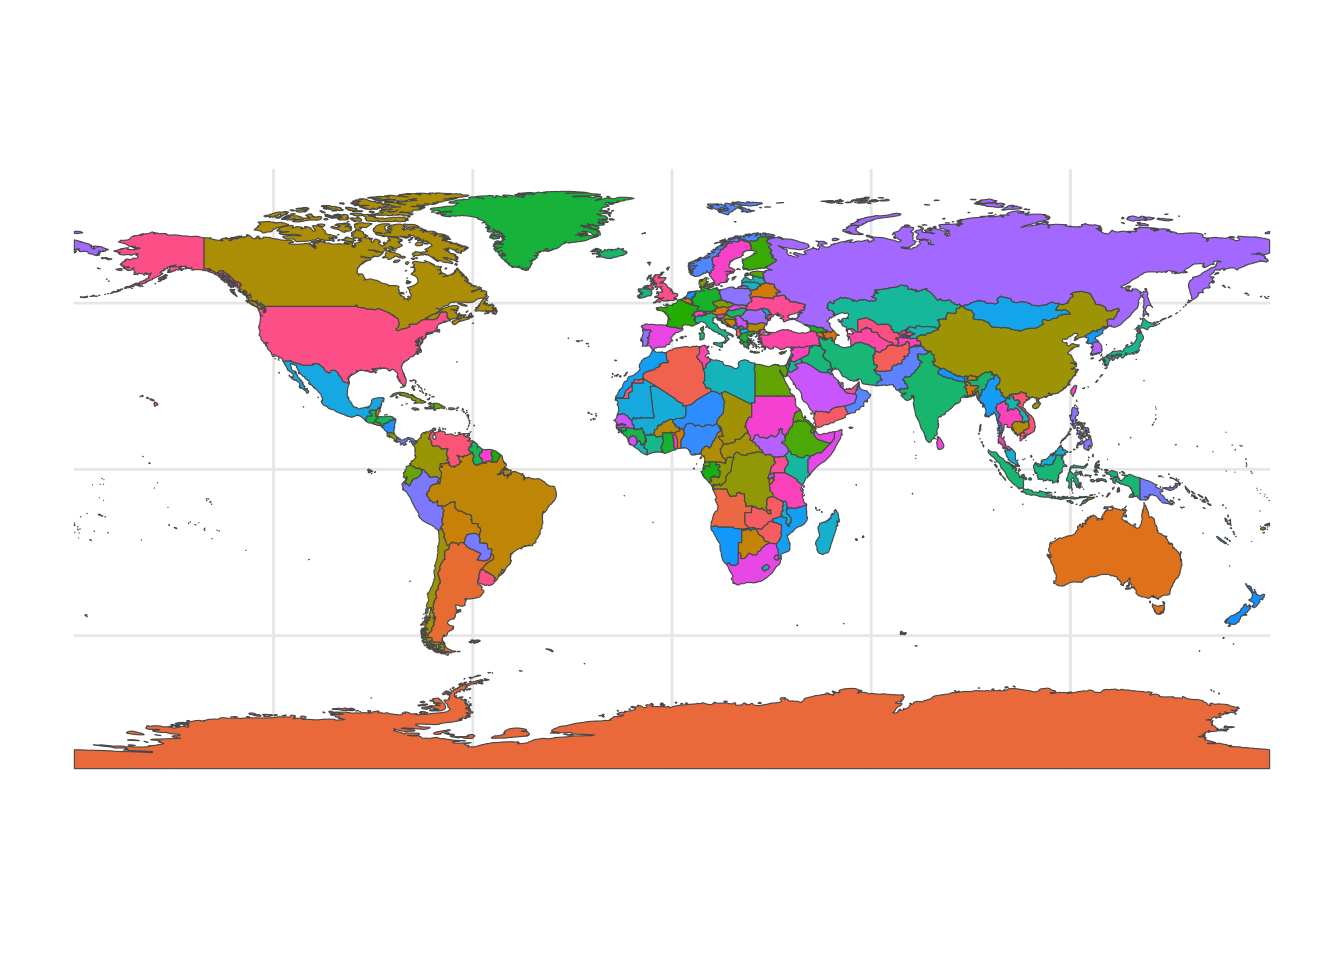
\includegraphics{maps-exercise_files/figure-latex/worldmap-1.pdf}

\begin{Shaded}
\begin{Highlighting}[]
\NormalTok{wmap\_ant }\OtherTok{\textless{}{-}} \FunctionTok{getMap}\NormalTok{()[}\SpecialCharTok{{-}}\FunctionTok{which}\NormalTok{(}\FunctionTok{getMap}\NormalTok{()}\SpecialCharTok{$}\NormalTok{ADMIN}\SpecialCharTok{==}\StringTok{\textquotesingle{}Antarctica\textquotesingle{}}\NormalTok{),]  }\SpecialCharTok{\%\textgreater{}\%}
  \FunctionTok{st\_as\_sf}\NormalTok{()}
\FunctionTok{ggplot}\NormalTok{(}\AttributeTok{data =}\NormalTok{ wmap\_ant) }\SpecialCharTok{+}
  \FunctionTok{geom\_sf}\NormalTok{(}\FunctionTok{aes}\NormalTok{(}\AttributeTok{fill =}\NormalTok{ NAME)) }\SpecialCharTok{+}
  \FunctionTok{theme\_minimal}\NormalTok{() }\SpecialCharTok{+}
  \FunctionTok{guides}\NormalTok{(}\AttributeTok{fill =} \ConstantTok{FALSE}\NormalTok{) }\CommentTok{\# don\textquotesingle{}t show legend}
\end{Highlighting}
\end{Shaded}

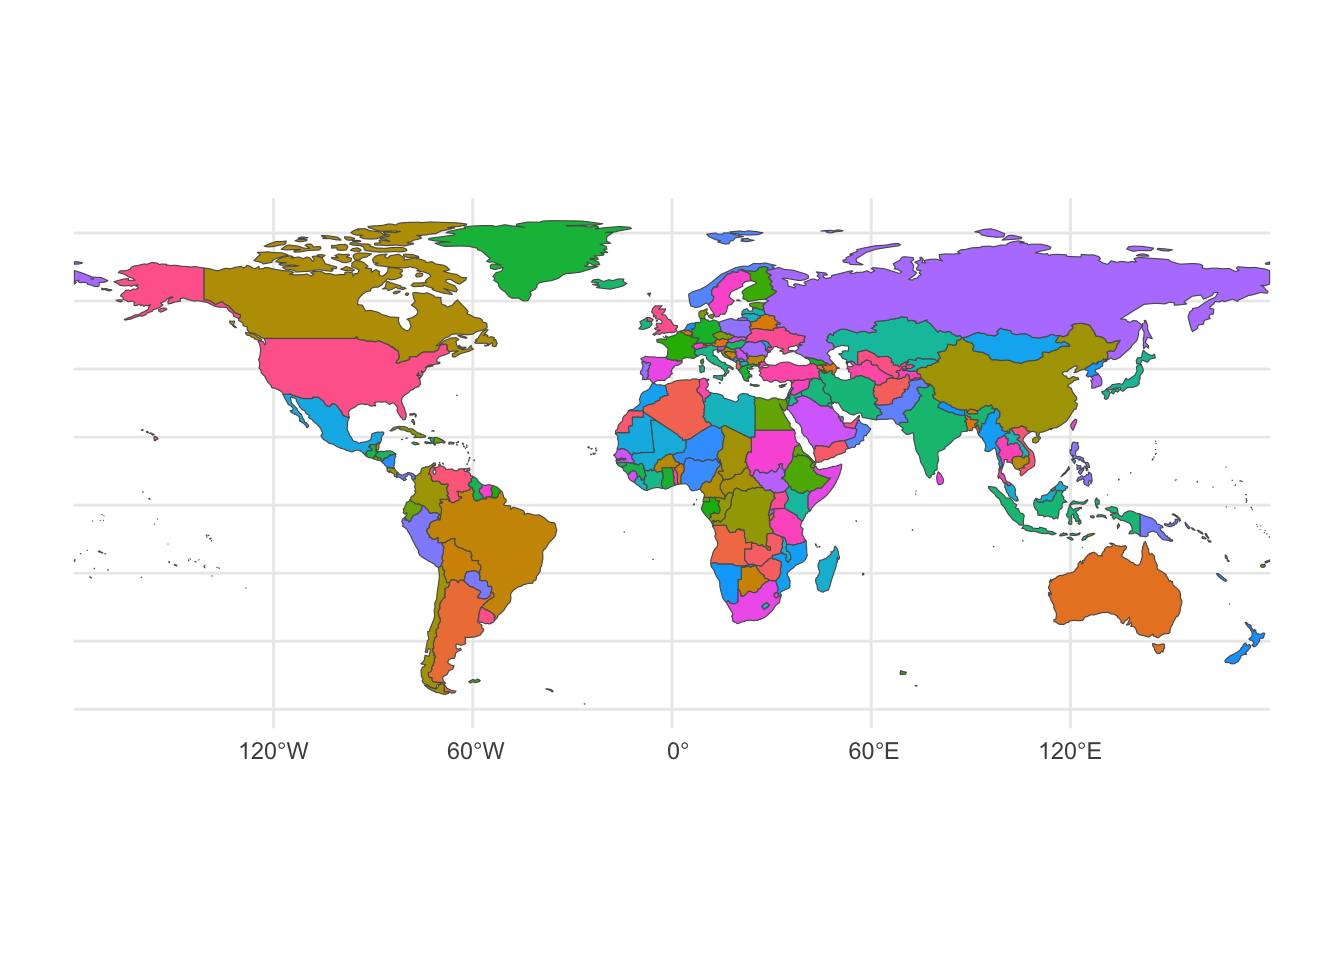
\includegraphics{maps-exercise_files/figure-latex/unnamed-chunk-1-1.pdf}

\hypertarget{raster-maps}{%
\section{Raster maps}\label{raster-maps}}

\hypertarget{simple-example-httpsggplot2.tidyverse.orgreferenceggsf.html}{%
\subsection{\texorpdfstring{Simple example:
\url{https://ggplot2.tidyverse.org/reference/ggsf.html}}{Simple example: https://ggplot2.tidyverse.org/reference/ggsf.html}}\label{simple-example-httpsggplot2.tidyverse.orgreferenceggsf.html}}

\begin{Shaded}
\begin{Highlighting}[]
\NormalTok{nc }\OtherTok{\textless{}{-}}\NormalTok{ sf}\SpecialCharTok{::}\FunctionTok{st\_read}\NormalTok{(}\FunctionTok{system.file}\NormalTok{(}\StringTok{"shape/nc.shp"}\NormalTok{, }\AttributeTok{package =} \StringTok{"sf"}\NormalTok{), }\AttributeTok{quiet =} \ConstantTok{TRUE}\NormalTok{)}
\FunctionTok{ggplot}\NormalTok{(nc) }\SpecialCharTok{+}
  \FunctionTok{geom\_sf}\NormalTok{(}\FunctionTok{aes}\NormalTok{(}\AttributeTok{fill =}\NormalTok{ AREA))}
\end{Highlighting}
\end{Shaded}

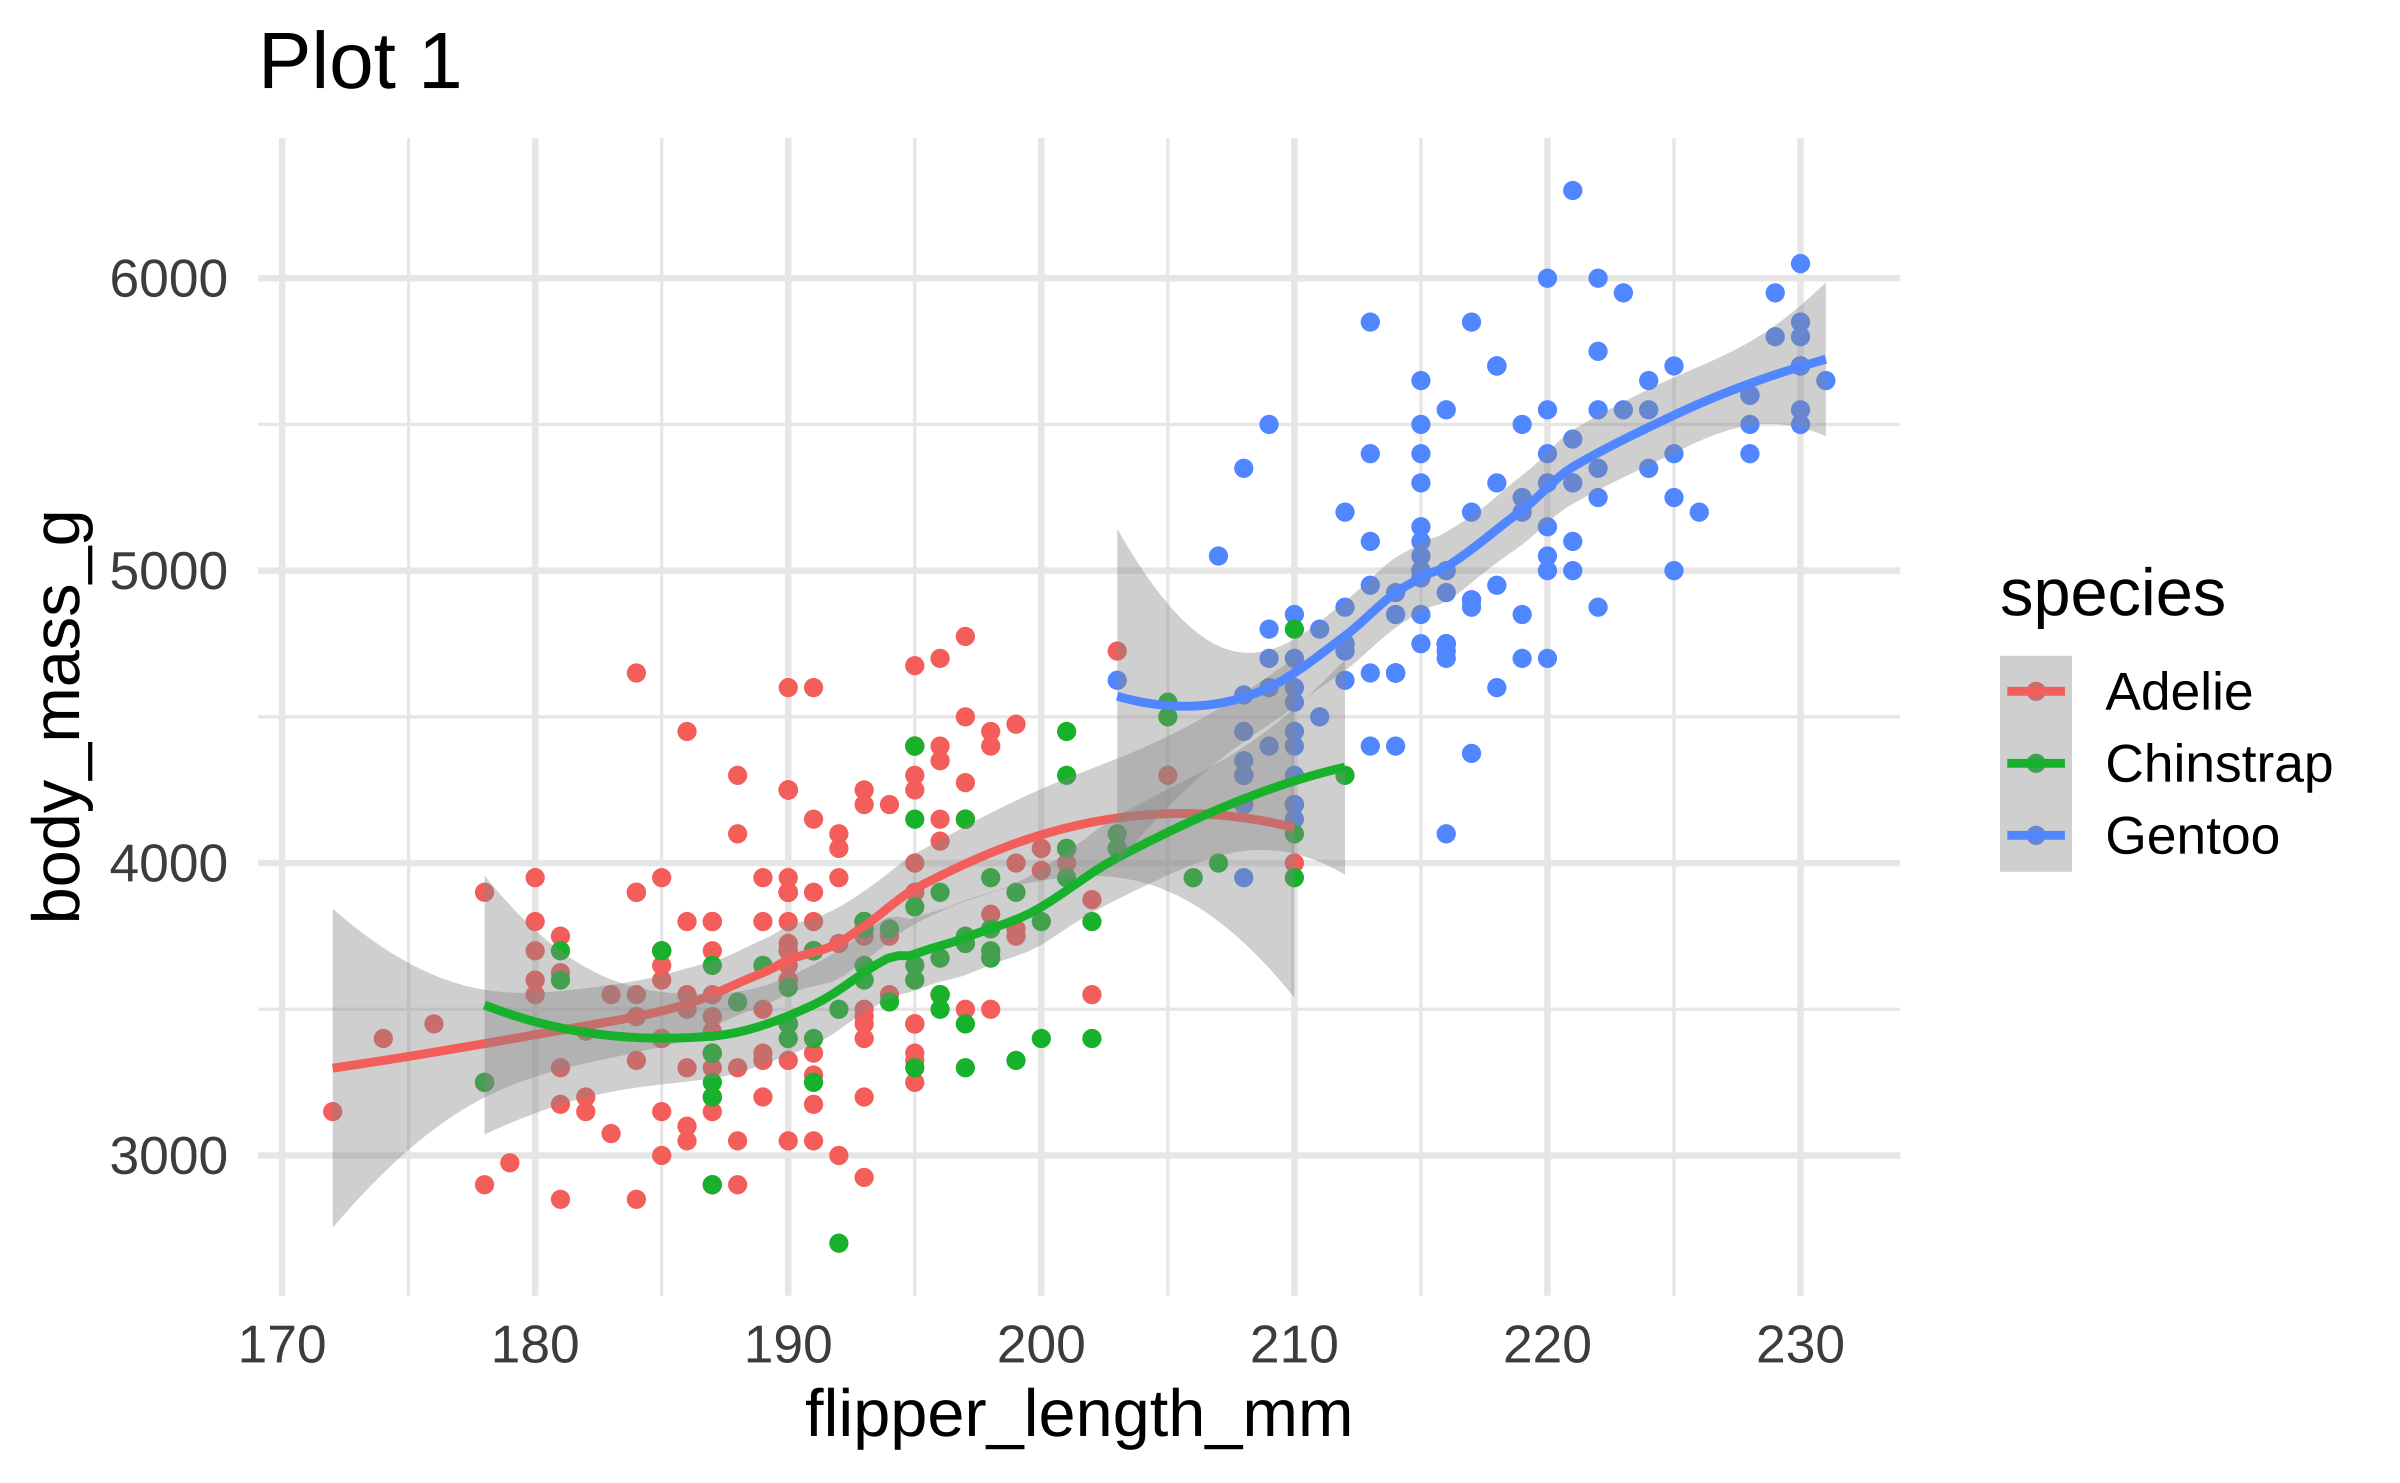
\includegraphics{maps-exercise_files/figure-latex/unnamed-chunk-2-1.pdf}

\begin{Shaded}
\begin{Highlighting}[]
\CommentTok{\# If not supplied, coord\_sf() will take the CRS from the first layer}
\CommentTok{\# and automatically transform all other layers to use that CRS. This}
\CommentTok{\# ensures that all data will correctly line up}
\NormalTok{nc\_3857 }\OtherTok{\textless{}{-}}\NormalTok{ sf}\SpecialCharTok{::}\FunctionTok{st\_transform}\NormalTok{(nc, }\DecValTok{3857}\NormalTok{)}
\FunctionTok{ggplot}\NormalTok{() }\SpecialCharTok{+}
  \FunctionTok{geom\_sf}\NormalTok{(}\AttributeTok{data =}\NormalTok{ nc) }\SpecialCharTok{+}
  \FunctionTok{geom\_sf}\NormalTok{(}\AttributeTok{data =}\NormalTok{ nc\_3857, }\AttributeTok{colour =} \StringTok{"red"}\NormalTok{, }\AttributeTok{fill =} \ConstantTok{NA}\NormalTok{)}
\end{Highlighting}
\end{Shaded}

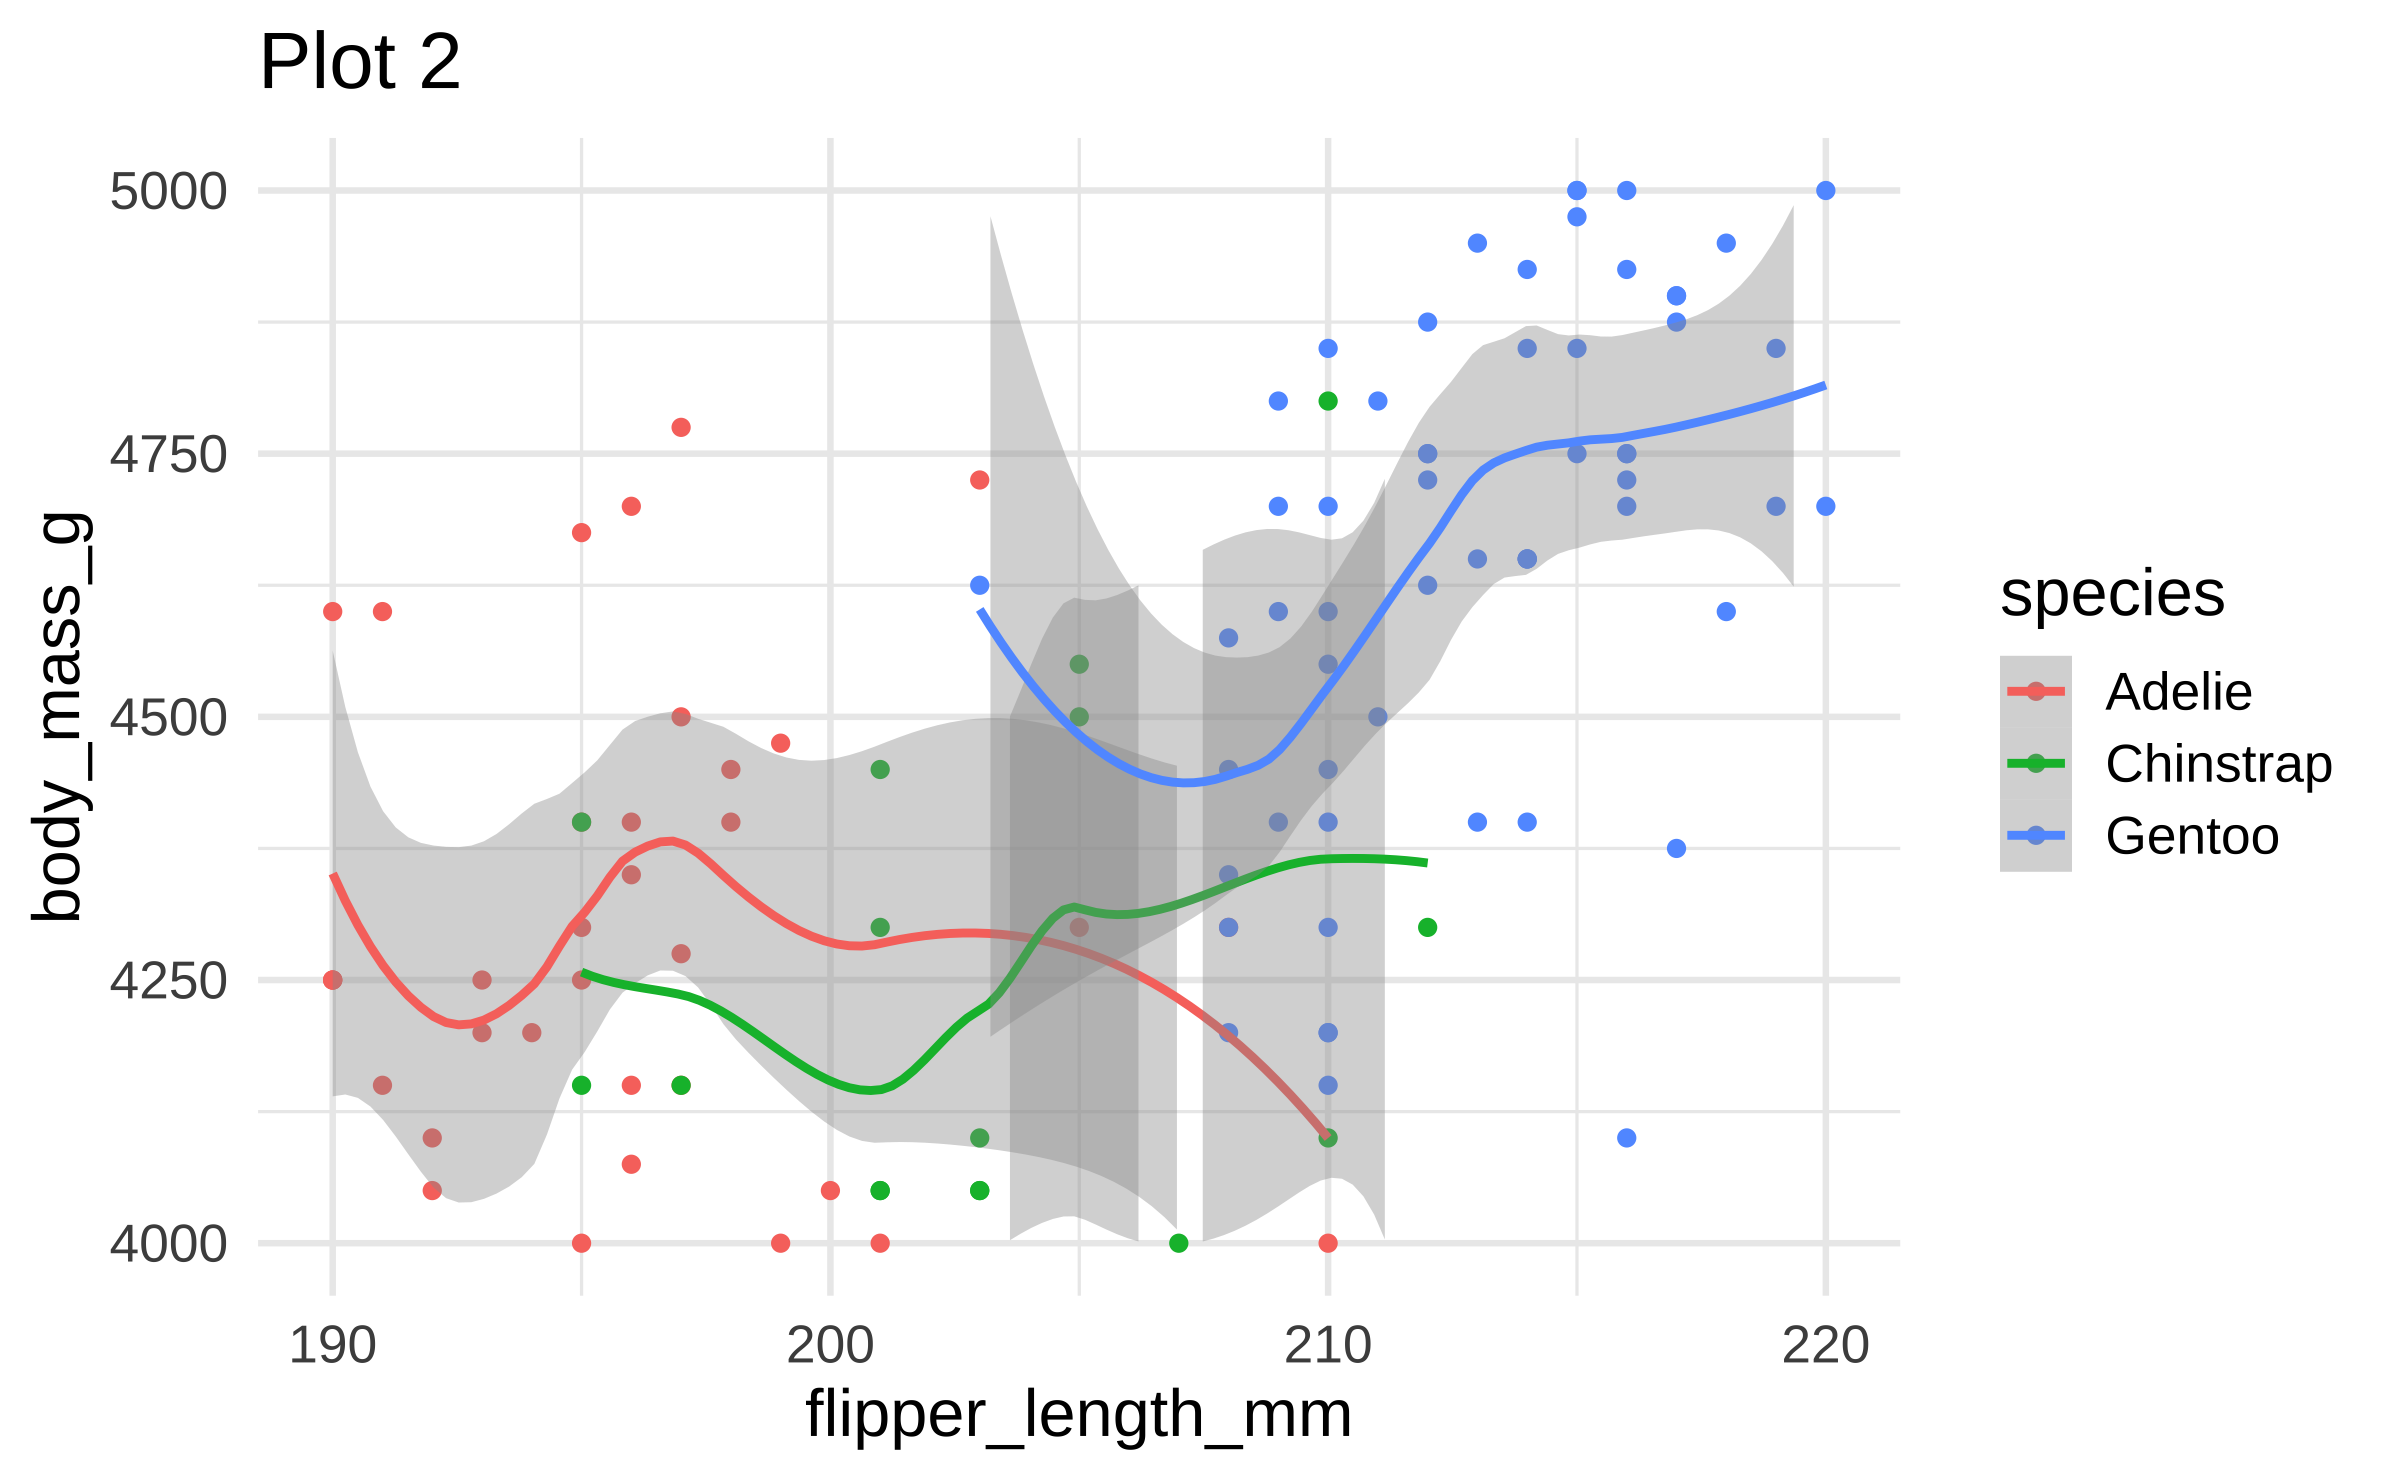
\includegraphics{maps-exercise_files/figure-latex/unnamed-chunk-2-2.pdf}

\begin{Shaded}
\begin{Highlighting}[]
\CommentTok{\# Unfortunately if you plot other types of feature you\textquotesingle{}ll need to use}
\CommentTok{\# show.legend to tell ggplot2 what type of legend to use}
\NormalTok{nc\_3857}\SpecialCharTok{$}\NormalTok{mid }\OtherTok{\textless{}{-}}\NormalTok{ sf}\SpecialCharTok{::}\FunctionTok{st\_centroid}\NormalTok{(nc\_3857}\SpecialCharTok{$}\NormalTok{geometry)}
\FunctionTok{ggplot}\NormalTok{(nc\_3857) }\SpecialCharTok{+}
  \FunctionTok{geom\_sf}\NormalTok{(}\AttributeTok{colour =} \StringTok{"white"}\NormalTok{) }\SpecialCharTok{+}
  \FunctionTok{geom\_sf}\NormalTok{(}\FunctionTok{aes}\NormalTok{(}\AttributeTok{geometry =}\NormalTok{ mid, }\AttributeTok{size =}\NormalTok{ AREA), }\AttributeTok{show.legend =} \StringTok{"point"}\NormalTok{)}
\end{Highlighting}
\end{Shaded}

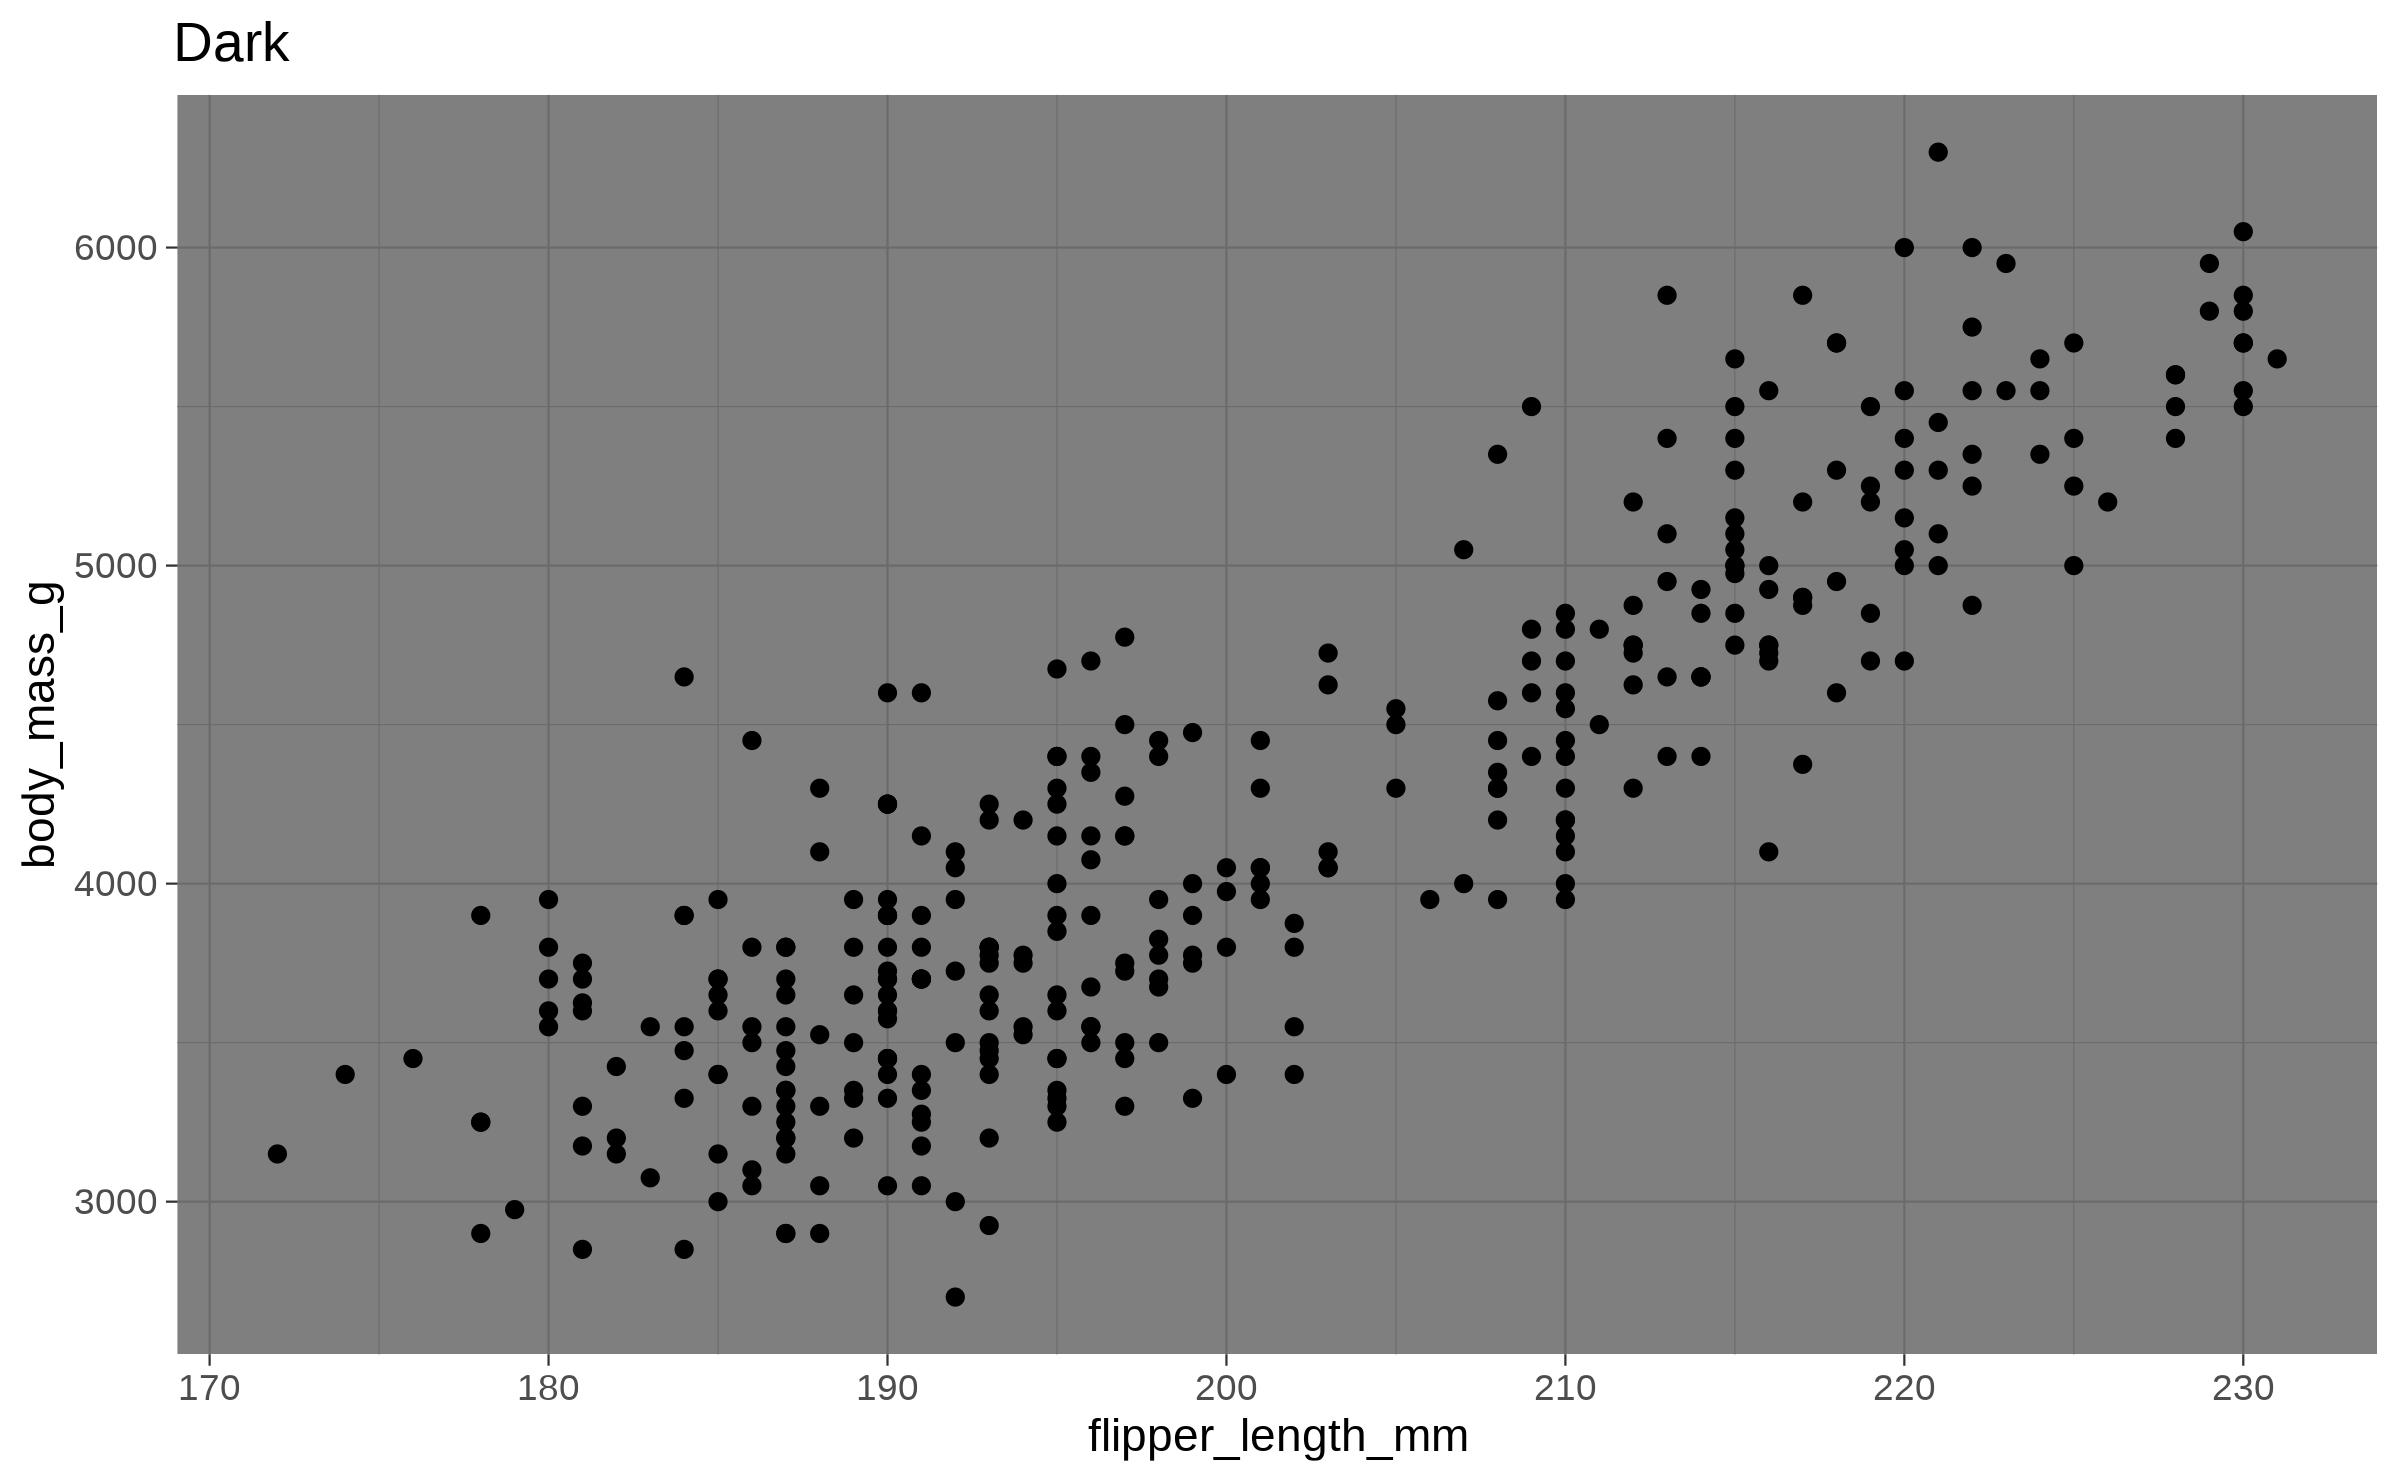
\includegraphics{maps-exercise_files/figure-latex/unnamed-chunk-2-3.pdf}

\begin{Shaded}
\begin{Highlighting}[]
\CommentTok{\# You can also use layers with x and y aesthetics. To have these interpreted}
\CommentTok{\# as longitude/latitude you need to set the default CRS in coord\_sf()}
\FunctionTok{ggplot}\NormalTok{(nc\_3857) }\SpecialCharTok{+}
  \FunctionTok{geom\_sf}\NormalTok{() }\SpecialCharTok{+}
  \FunctionTok{annotate}\NormalTok{(}\StringTok{"point"}\NormalTok{, }\AttributeTok{x =} \SpecialCharTok{{-}}\DecValTok{80}\NormalTok{, }\AttributeTok{y =} \DecValTok{35}\NormalTok{, }\AttributeTok{colour =} \StringTok{"red"}\NormalTok{, }\AttributeTok{size =} \DecValTok{4}\NormalTok{) }\SpecialCharTok{+}
  \FunctionTok{coord\_sf}\NormalTok{(}\AttributeTok{default\_crs =}\NormalTok{ sf}\SpecialCharTok{::}\FunctionTok{st\_crs}\NormalTok{(}\DecValTok{4326}\NormalTok{))}
\end{Highlighting}
\end{Shaded}

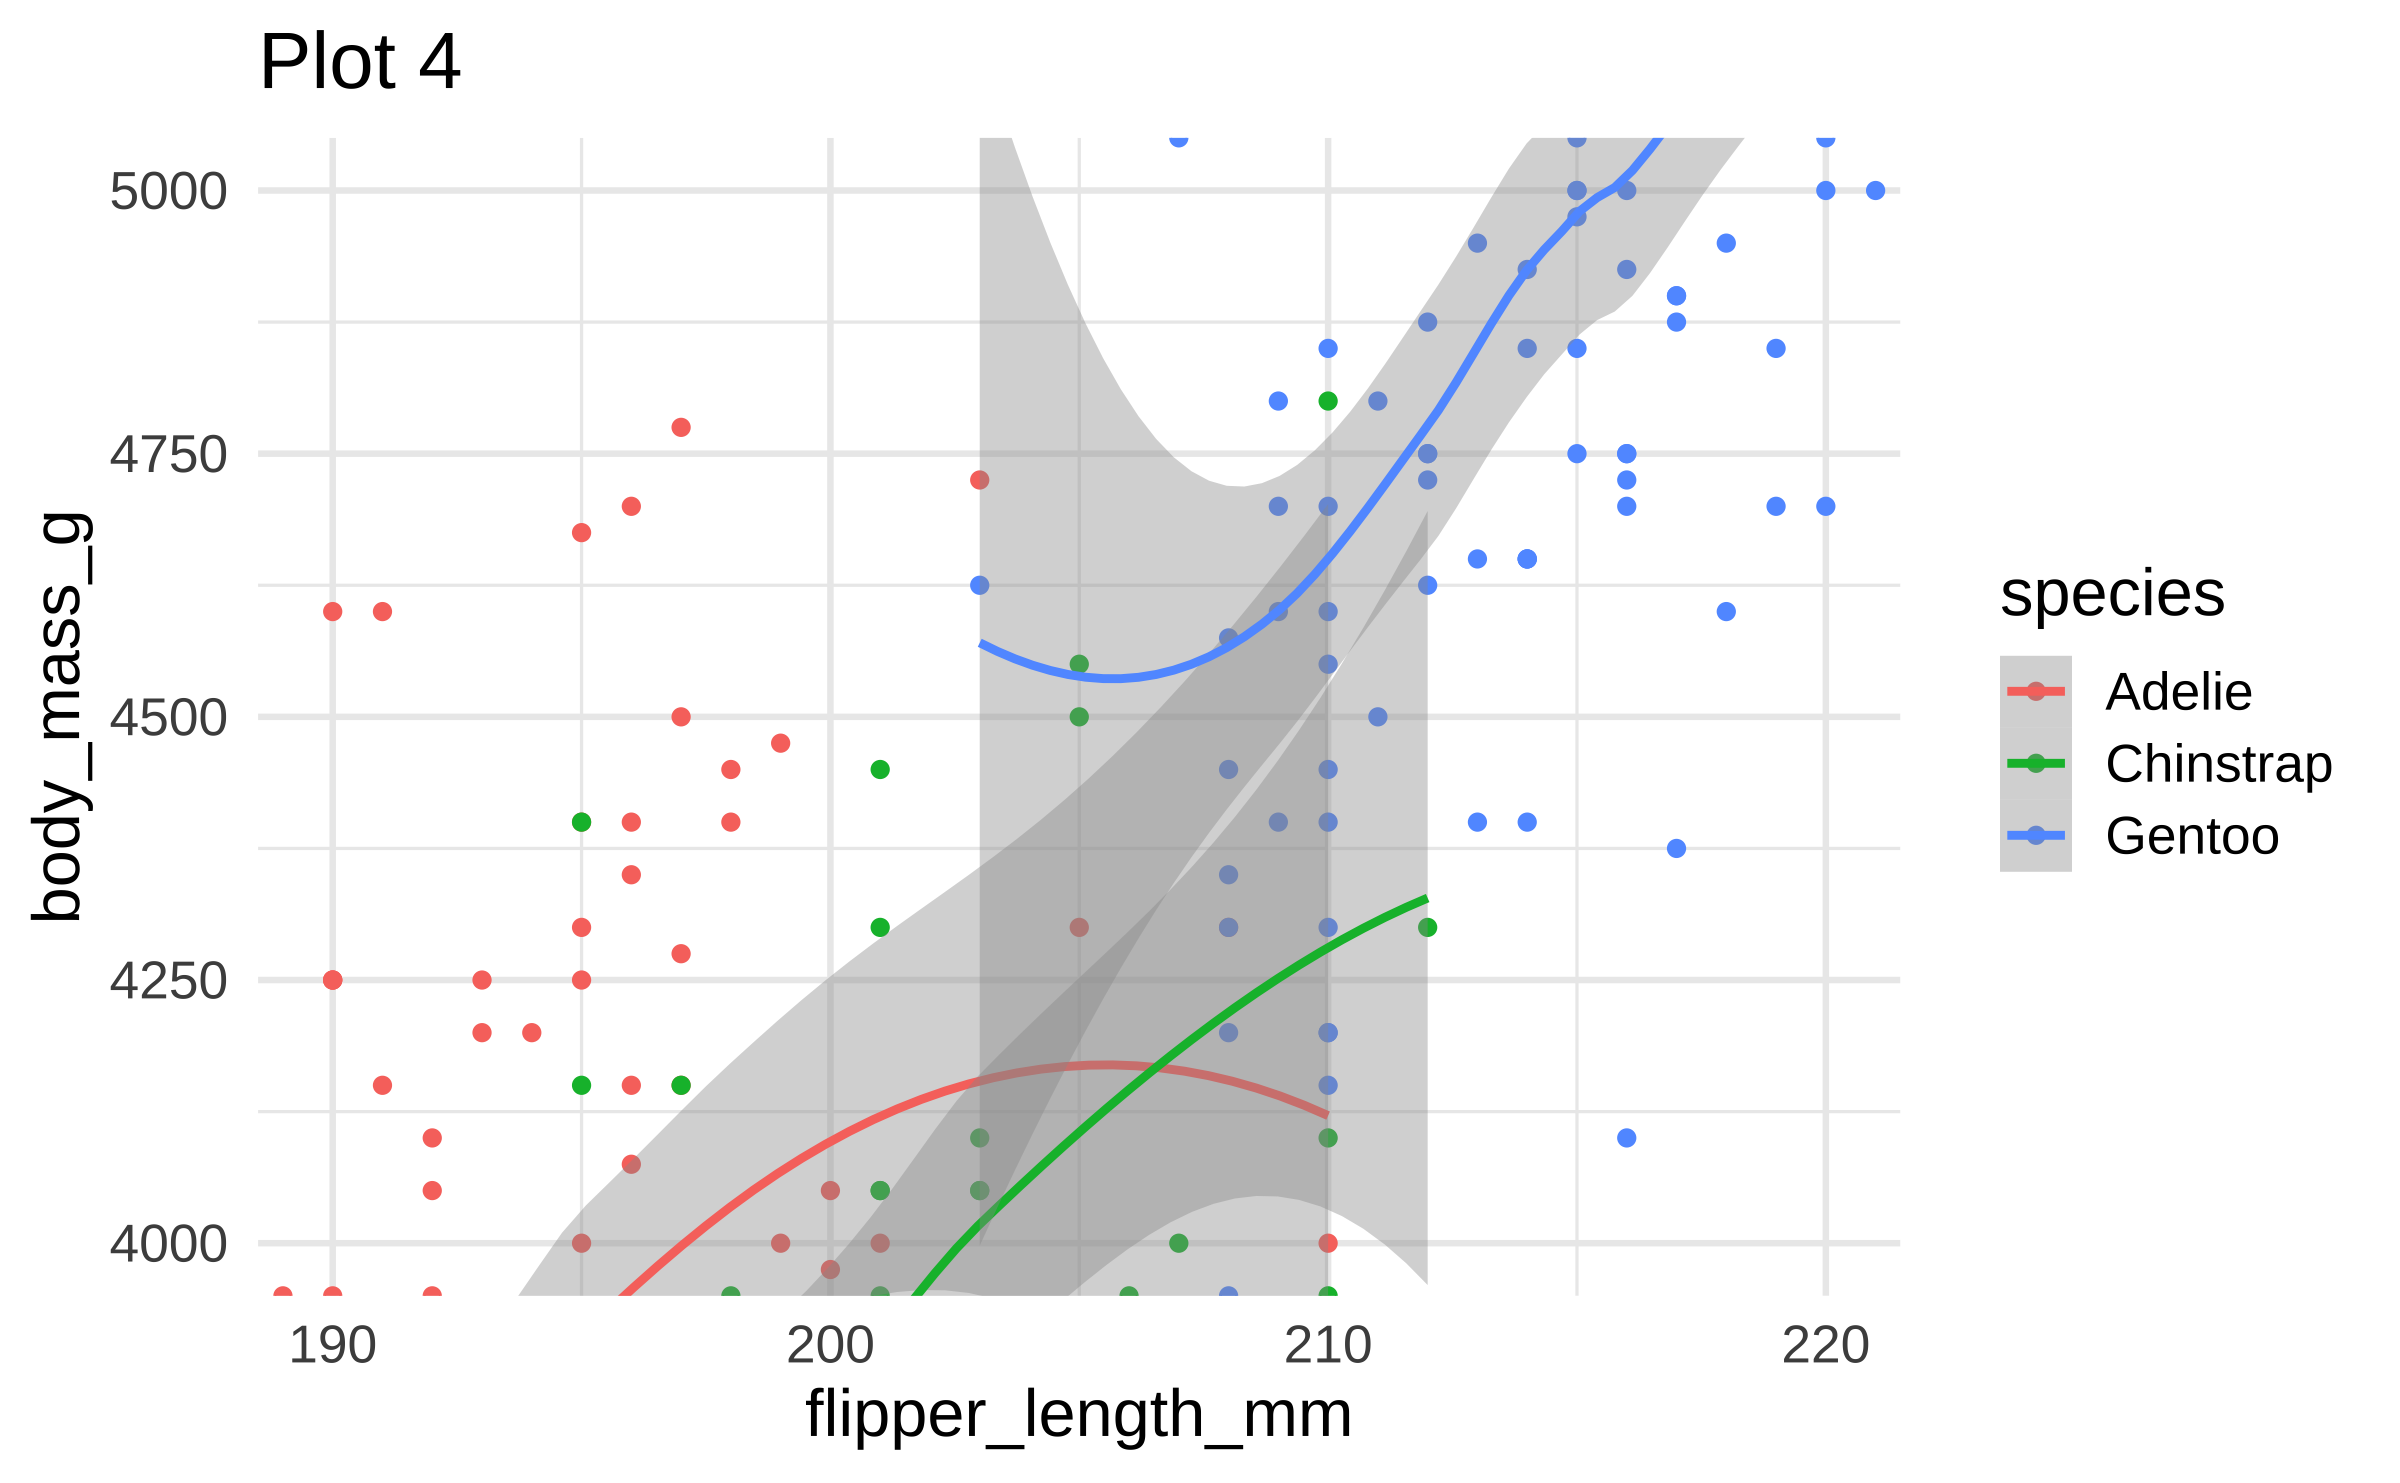
\includegraphics{maps-exercise_files/figure-latex/unnamed-chunk-2-4.pdf}

\begin{Shaded}
\begin{Highlighting}[]
\CommentTok{\# To add labels, use geom\_sf\_label().}
\FunctionTok{ggplot}\NormalTok{(nc\_3857[}\DecValTok{1}\SpecialCharTok{:}\DecValTok{3}\NormalTok{, ]) }\SpecialCharTok{+}
   \FunctionTok{geom\_sf}\NormalTok{(}\FunctionTok{aes}\NormalTok{(}\AttributeTok{fill =}\NormalTok{ AREA)) }\SpecialCharTok{+}
   \FunctionTok{geom\_sf\_label}\NormalTok{(}\FunctionTok{aes}\NormalTok{(}\AttributeTok{label =}\NormalTok{ NAME))}
\end{Highlighting}
\end{Shaded}

\includegraphics{maps-exercise_files/figure-latex/unnamed-chunk-2-5.pdf}

\hypertarget{illinois-example}{%
\subsection{Illinois example}\label{illinois-example}}

\begin{Shaded}
\begin{Highlighting}[]
\NormalTok{il\_counties }\OtherTok{\textless{}{-}} \FunctionTok{map\_data}\NormalTok{(}\StringTok{"county"}\NormalTok{, }\StringTok{"illinois"}\NormalTok{) }
\FunctionTok{head}\NormalTok{(il\_counties)}
\end{Highlighting}
\end{Shaded}

\begin{verbatim}
##        long      lat group order   region subregion
## 1 -91.49563 40.21018     1     1 illinois     adams
## 2 -90.91121 40.19299     1     2 illinois     adams
## 3 -90.91121 40.19299     1     3 illinois     adams
## 4 -90.91121 40.10704     1     4 illinois     adams
## 5 -90.91121 39.83775     1     5 illinois     adams
## 6 -90.91694 39.75754     1     6 illinois     adams
\end{verbatim}

\begin{Shaded}
\begin{Highlighting}[]
\FunctionTok{ggplot}\NormalTok{(il\_counties, }\FunctionTok{aes}\NormalTok{(long, lat, }\AttributeTok{group =}\NormalTok{ group)) }\SpecialCharTok{+}
  \FunctionTok{geom\_polygon}\NormalTok{(}\AttributeTok{fill =} \StringTok{"white"}\NormalTok{, }\AttributeTok{colour =} \StringTok{"grey50"}\NormalTok{) }\SpecialCharTok{+} 
  \FunctionTok{coord\_quickmap}\NormalTok{()}
\end{Highlighting}
\end{Shaded}

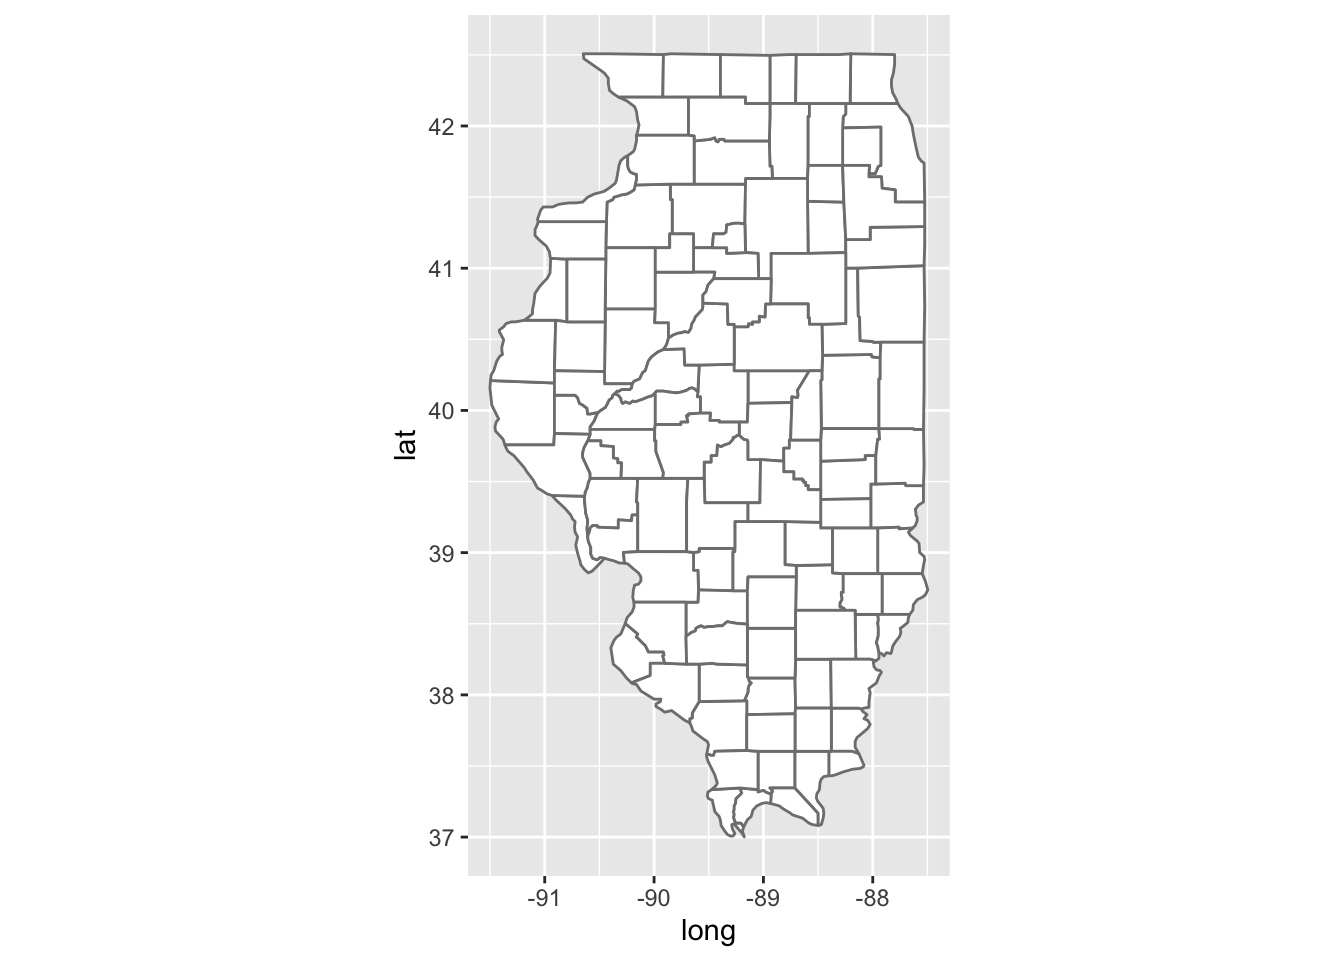
\includegraphics{maps-exercise_files/figure-latex/map-il-1.pdf}

\begin{Shaded}
\begin{Highlighting}[]
\NormalTok{il\_county }\OtherTok{\textless{}{-}}\NormalTok{ tigris}\SpecialCharTok{::}\FunctionTok{counties}\NormalTok{(}\AttributeTok{state =} \StringTok{"illinois"}\NormalTok{, }\AttributeTok{cb =} \ConstantTok{TRUE}\NormalTok{) }\SpecialCharTok{\%\textgreater{}\%} 
    \FunctionTok{st\_as\_sf}\NormalTok{() }
\end{Highlighting}
\end{Shaded}

\begin{verbatim}
##   |                                                                              |                                                                      |   0%  |                                                                              |                                                                      |   1%  |                                                                              |=                                                                     |   1%  |                                                                              |=                                                                     |   2%  |                                                                              |==                                                                    |   2%  |                                                                              |==                                                                    |   3%  |                                                                              |===                                                                   |   4%  |                                                                              |====                                                                  |   5%  |                                                                              |====                                                                  |   6%  |                                                                              |=====                                                                 |   6%  |                                                                              |=====                                                                 |   7%  |                                                                              |======                                                                |   8%  |                                                                              |======                                                                |   9%  |                                                                              |========                                                              |  11%  |                                                                              |=========                                                             |  12%  |                                                                              |=========                                                             |  13%  |                                                                              |==========                                                            |  14%  |                                                                              |===========                                                           |  15%  |                                                                              |===========                                                           |  16%  |                                                                              |============                                                          |  17%  |                                                                              |============                                                          |  18%  |                                                                              |=============                                                         |  18%  |                                                                              |=============                                                         |  19%  |                                                                              |==============                                                        |  19%  |                                                                              |==============                                                        |  20%  |                                                                              |===============                                                       |  21%  |                                                                              |===============                                                       |  22%  |                                                                              |================                                                      |  23%  |                                                                              |=================                                                     |  24%  |                                                                              |=================                                                     |  25%  |                                                                              |==================                                                    |  25%  |                                                                              |==================                                                    |  26%  |                                                                              |===================                                                   |  26%  |                                                                              |===================                                                   |  27%  |                                                                              |===================                                                   |  28%  |                                                                              |====================                                                  |  28%  |                                                                              |====================                                                  |  29%  |                                                                              |=====================                                                 |  29%  |                                                                              |=====================                                                 |  30%  |                                                                              |=====================                                                 |  31%  |                                                                              |======================                                                |  31%  |                                                                              |=======================                                               |  33%  |                                                                              |=========================                                             |  35%  |                                                                              |============================                                          |  40%  |                                                                              |=============================                                         |  42%  |                                                                              |===============================                                       |  44%  |                                                                              |========================================                              |  58%  |                                                                              |=========================================                             |  59%  |                                                                              |==============================================                        |  66%  |                                                                              |===================================================                   |  73%  |                                                                              |===========================================================           |  85%  |                                                                              |================================================================      |  92%  |                                                                              |==================================================================    |  94%  |                                                                              |======================================================================| 100%
\end{verbatim}

\begin{Shaded}
\begin{Highlighting}[]
\FunctionTok{ggplot}\NormalTok{(il\_county) }\SpecialCharTok{+} 
  \FunctionTok{geom\_sf}\NormalTok{(}\AttributeTok{color =} \StringTok{"blue"}\NormalTok{, }\AttributeTok{fill =} \StringTok{"lightgray"}\NormalTok{) }
\end{Highlighting}
\end{Shaded}

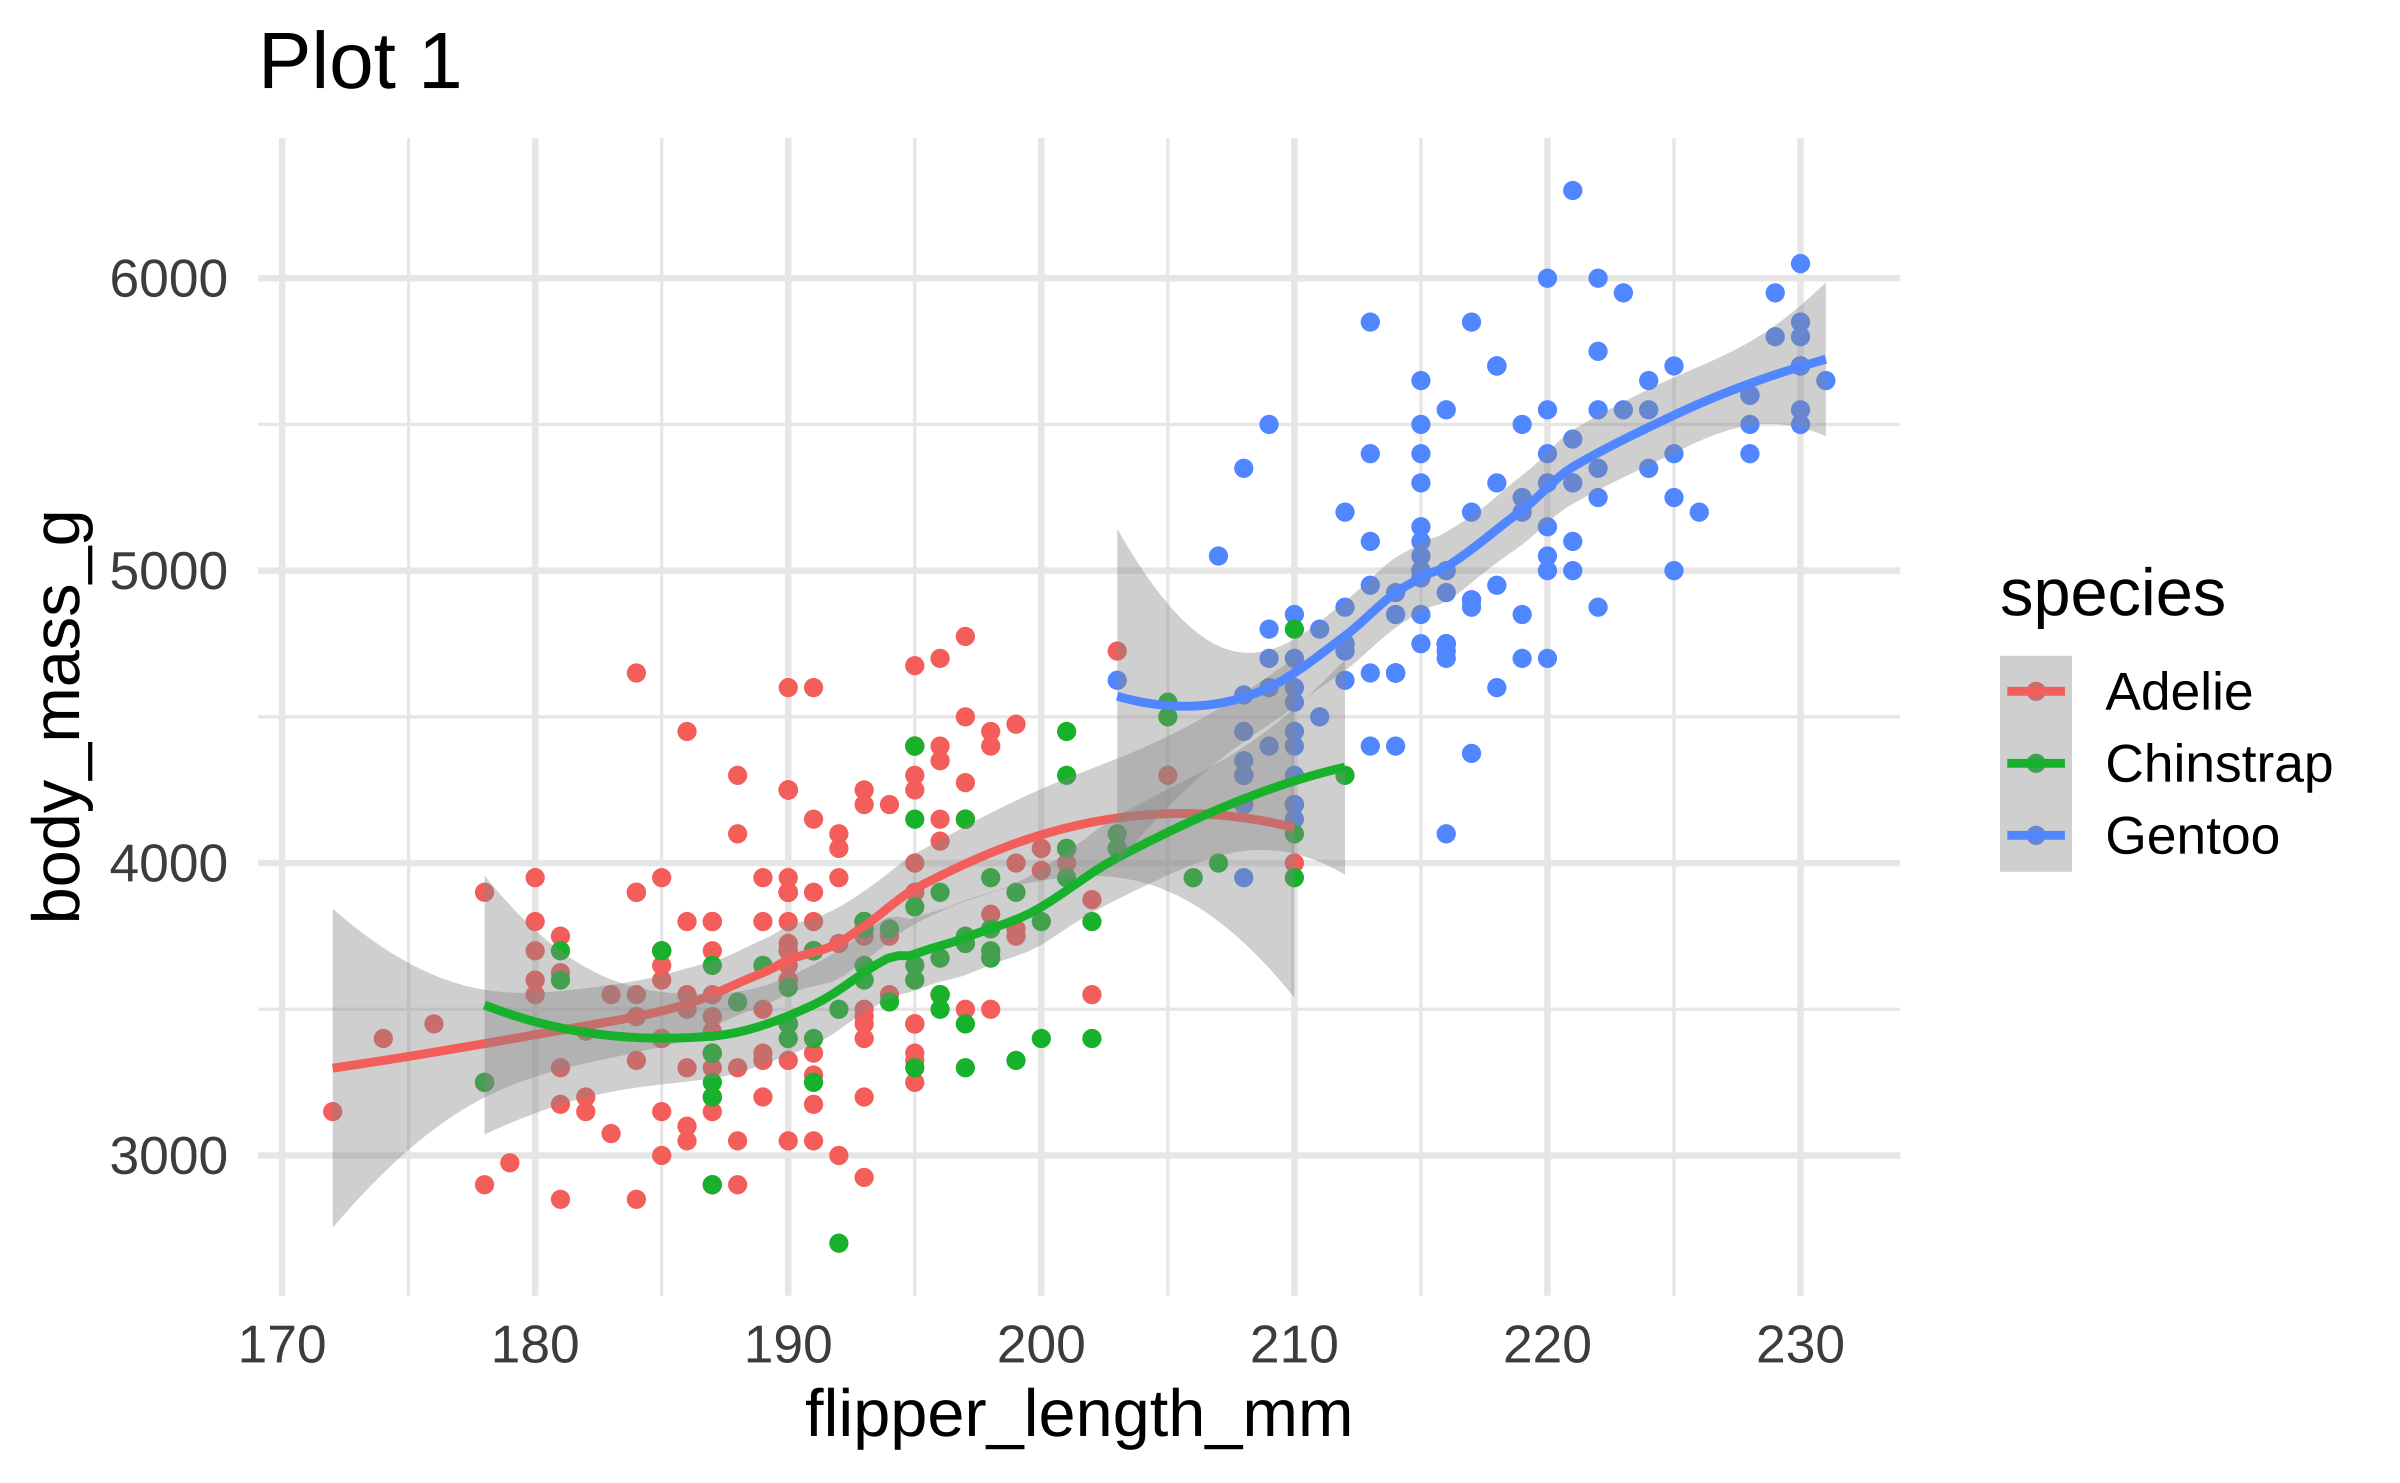
\includegraphics{maps-exercise_files/figure-latex/unnamed-chunk-3-1.pdf}

\hypertarget{add-cities}{%
\subsection{Add cities}\label{add-cities}}

\emph{Data source: \url{https://geo-csv.com/illinois/}}

\begin{Shaded}
\begin{Highlighting}[]
\NormalTok{illinois }\OtherTok{\textless{}{-}} \FunctionTok{read\_csv}\NormalTok{(}\StringTok{"../data/illinois.csv"}\NormalTok{)}
\end{Highlighting}
\end{Shaded}

\begin{verbatim}
## Rows: 5272 Columns: 3
## -- Column specification --------------------------------------------------------
## Delimiter: ","
## chr (1): city_name
## dbl (2): city_latitude, city_longitude
## 
## i Use `spec()` to retrieve the full column specification for this data.
## i Specify the column types or set `show_col_types = FALSE` to quiet this message.
\end{verbatim}

\begin{Shaded}
\begin{Highlighting}[]
\FunctionTok{ggplot}\NormalTok{(il\_county) }\SpecialCharTok{+} 
  \FunctionTok{geom\_sf}\NormalTok{(}\AttributeTok{color =} \StringTok{"blue"}\NormalTok{, }\AttributeTok{fill =} \StringTok{"gray"}\NormalTok{) }\SpecialCharTok{+}
 \FunctionTok{geom\_point}\NormalTok{(}\AttributeTok{data =}\NormalTok{ illinois, }
            \FunctionTok{aes}\NormalTok{(}\AttributeTok{x =}\NormalTok{ city\_longitude, }\AttributeTok{y =}\NormalTok{ city\_latitude), }
            \AttributeTok{colour =} \StringTok{"darkblue"}\NormalTok{, }\AttributeTok{size =} \FloatTok{0.1}\NormalTok{, }\AttributeTok{alpha =} \FloatTok{0.4}\NormalTok{) }\SpecialCharTok{+} 
  \FunctionTok{coord\_sf}\NormalTok{() }
\end{Highlighting}
\end{Shaded}

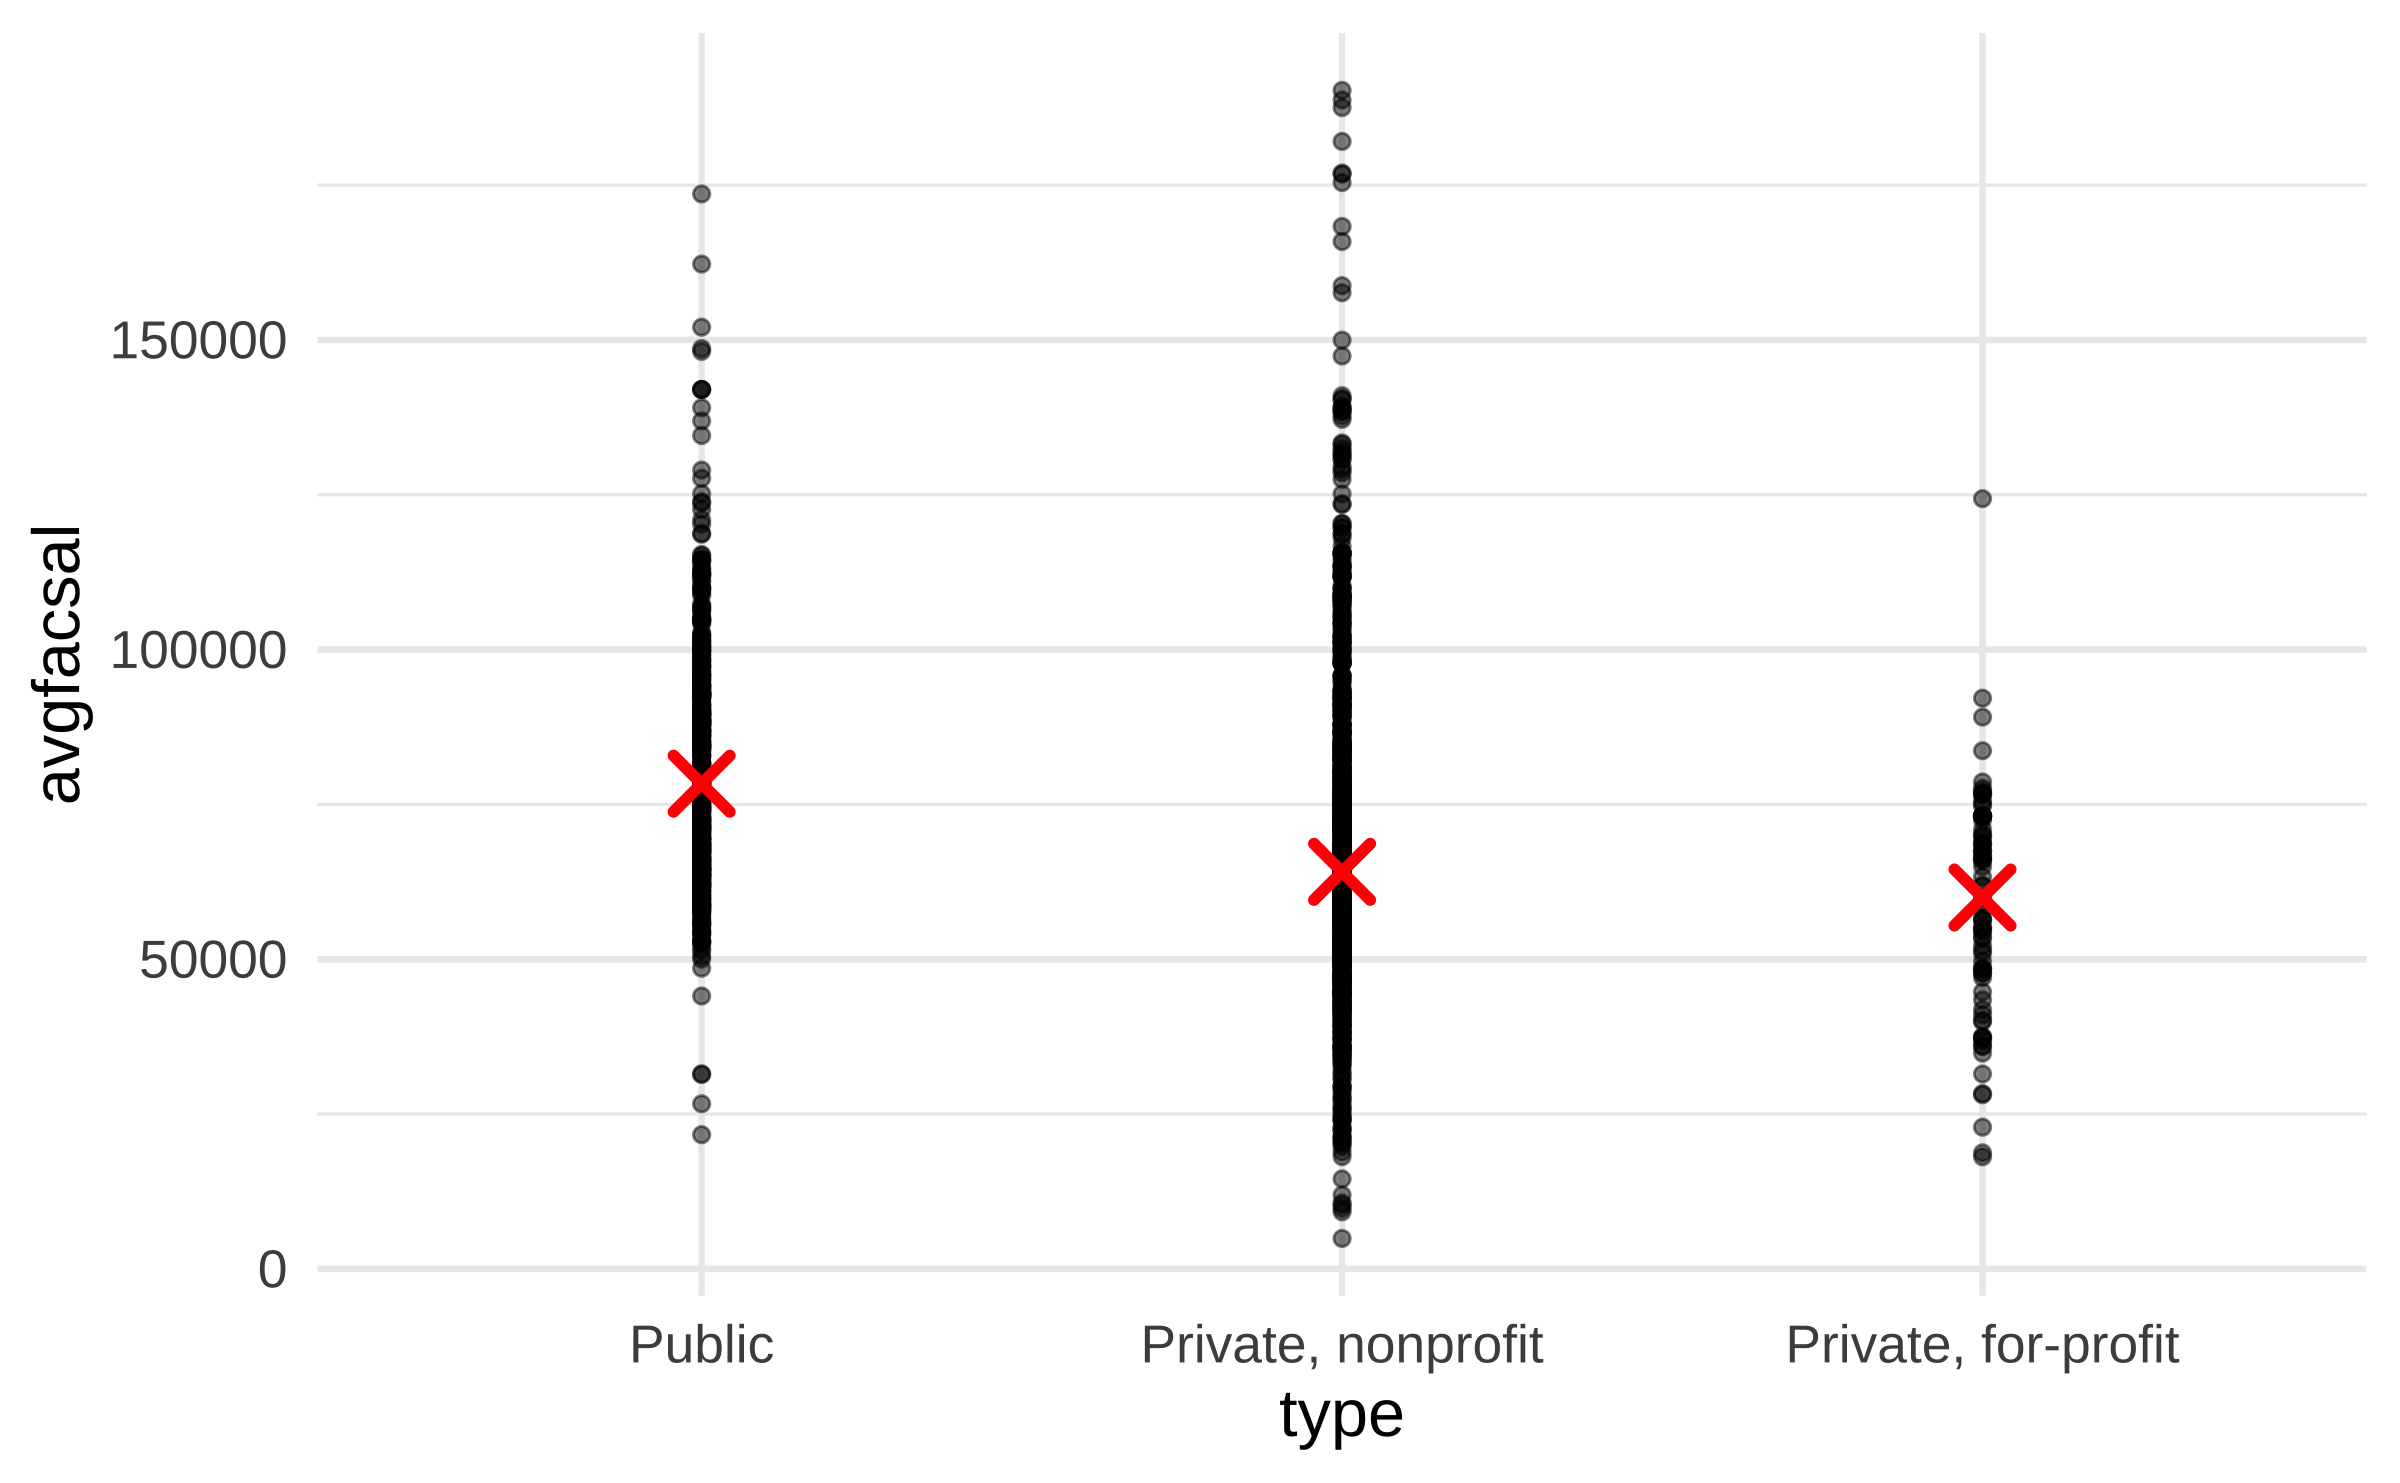
\includegraphics{maps-exercise_files/figure-latex/unnamed-chunk-4-1.pdf}

\begin{Shaded}
\begin{Highlighting}[]
\CommentTok{\# bring in county pop + cities}
\NormalTok{pop }\OtherTok{\textless{}{-}} \FunctionTok{read\_csv}\NormalTok{(}\StringTok{"../data/dceo\_county\_pop.csv"}\NormalTok{)}
\end{Highlighting}
\end{Shaded}

\begin{verbatim}
## Rows: 28119 Columns: 11
## -- Column specification --------------------------------------------------------
## Delimiter: ","
## chr (4): State/County, Race, Age Group, Sex
## dbl (7): 2000, 2005, 2010, 2015, 2020, 2025, 2030
## 
## i Use `spec()` to retrieve the full column specification for this data.
## i Specify the column types or set `show_col_types = FALSE` to quiet this message.
\end{verbatim}

\begin{Shaded}
\begin{Highlighting}[]
\CommentTok{\# merge by county}
\NormalTok{pop\_all }\OtherTok{\textless{}{-}}\NormalTok{ pop }\SpecialCharTok{\%\textgreater{}\%} \FunctionTok{filter}\NormalTok{(}\StringTok{\textasciigrave{}}\AttributeTok{Age Group}\StringTok{\textasciigrave{}} \SpecialCharTok{==} \StringTok{"All"} \SpecialCharTok{\&}\NormalTok{ Race }\SpecialCharTok{==} \StringTok{"All"}\NormalTok{) }\SpecialCharTok{\%\textgreater{}\%} \FunctionTok{mutate}\NormalTok{(}\AttributeTok{NAME =} \StringTok{\textasciigrave{}}\AttributeTok{State/County}\StringTok{\textasciigrave{}}\NormalTok{)}
\NormalTok{county\_pop }\OtherTok{\textless{}{-}} \FunctionTok{full\_join}\NormalTok{(il\_county, pop\_all, }\AttributeTok{by=}\StringTok{"NAME"}\NormalTok{)}
  
\CommentTok{\# plot}
\FunctionTok{ggplot}\NormalTok{() }\SpecialCharTok{+} \CommentTok{\# set up basic plot (don\textquotesingle{}t specify data b/c using two data sources)}
 \FunctionTok{geom\_sf}\NormalTok{(}\AttributeTok{data =}\NormalTok{ county\_pop, }\FunctionTok{aes}\NormalTok{(}\AttributeTok{fill =} \StringTok{\textasciigrave{}}\AttributeTok{2005}\StringTok{\textasciigrave{}}\NormalTok{)) }\SpecialCharTok{+} \CommentTok{\# setup our county data}
 \FunctionTok{scale\_fill\_continuous\_sequential}\NormalTok{(}\AttributeTok{palette =} \StringTok{"viridis"}\NormalTok{, }\AttributeTok{rev =} \ConstantTok{FALSE}\NormalTok{) }\SpecialCharTok{+}
  \FunctionTok{coord\_sf}\NormalTok{() }
\end{Highlighting}
\end{Shaded}

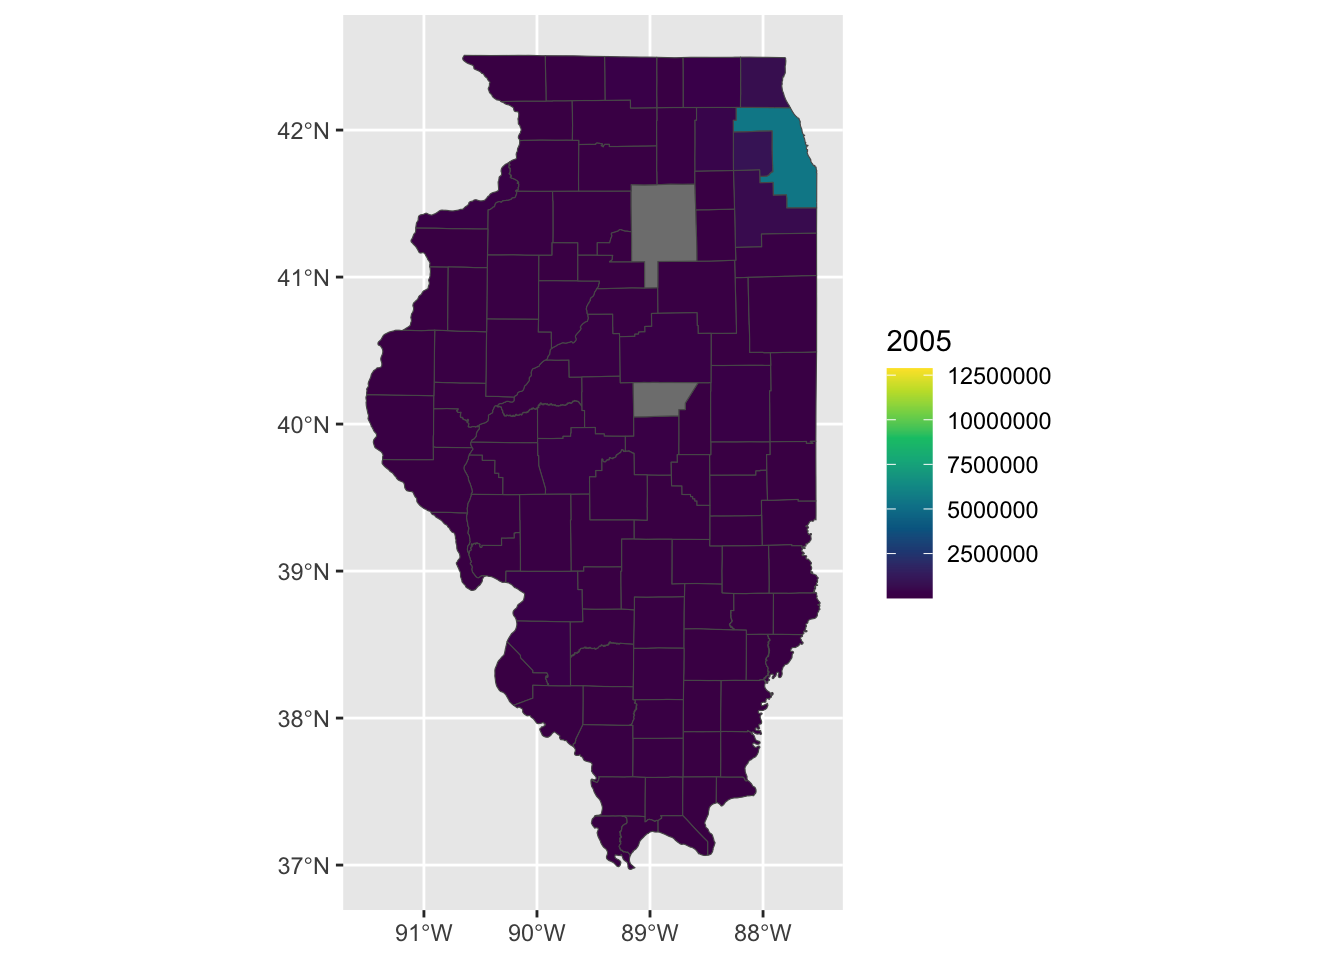
\includegraphics{maps-exercise_files/figure-latex/pop-1.pdf}

\begin{Shaded}
\begin{Highlighting}[]
\CommentTok{\#try breaks}
\FunctionTok{ggplot}\NormalTok{() }\SpecialCharTok{+} \CommentTok{\# set up basic plot (don\textquotesingle{}t specify data b/c using two data sources)}
 \FunctionTok{geom\_sf}\NormalTok{(}\AttributeTok{data =}\NormalTok{ county\_pop, }\FunctionTok{aes}\NormalTok{(}\AttributeTok{fill =} \StringTok{\textasciigrave{}}\AttributeTok{2005}\StringTok{\textasciigrave{}}\NormalTok{)) }\SpecialCharTok{+} \CommentTok{\# setup our county data}
 \FunctionTok{scale\_fill\_binned\_sequential}\NormalTok{(}
    \AttributeTok{palette =} \StringTok{"viridis"}\NormalTok{,}
    \AttributeTok{rev =} \ConstantTok{FALSE}\NormalTok{,}
    \AttributeTok{aesthetics =} \FunctionTok{c}\NormalTok{(}\StringTok{"fill"}\NormalTok{, }\StringTok{"color"}\NormalTok{),}
    \AttributeTok{n.breaks =} \DecValTok{3}\NormalTok{, }
\NormalTok{  ) }\SpecialCharTok{+}
  \FunctionTok{labs}\NormalTok{(}\AttributeTok{fill=}\StringTok{"2005 population"}\NormalTok{) }\SpecialCharTok{+} 
  \FunctionTok{coord\_sf}\NormalTok{() }
\end{Highlighting}
\end{Shaded}

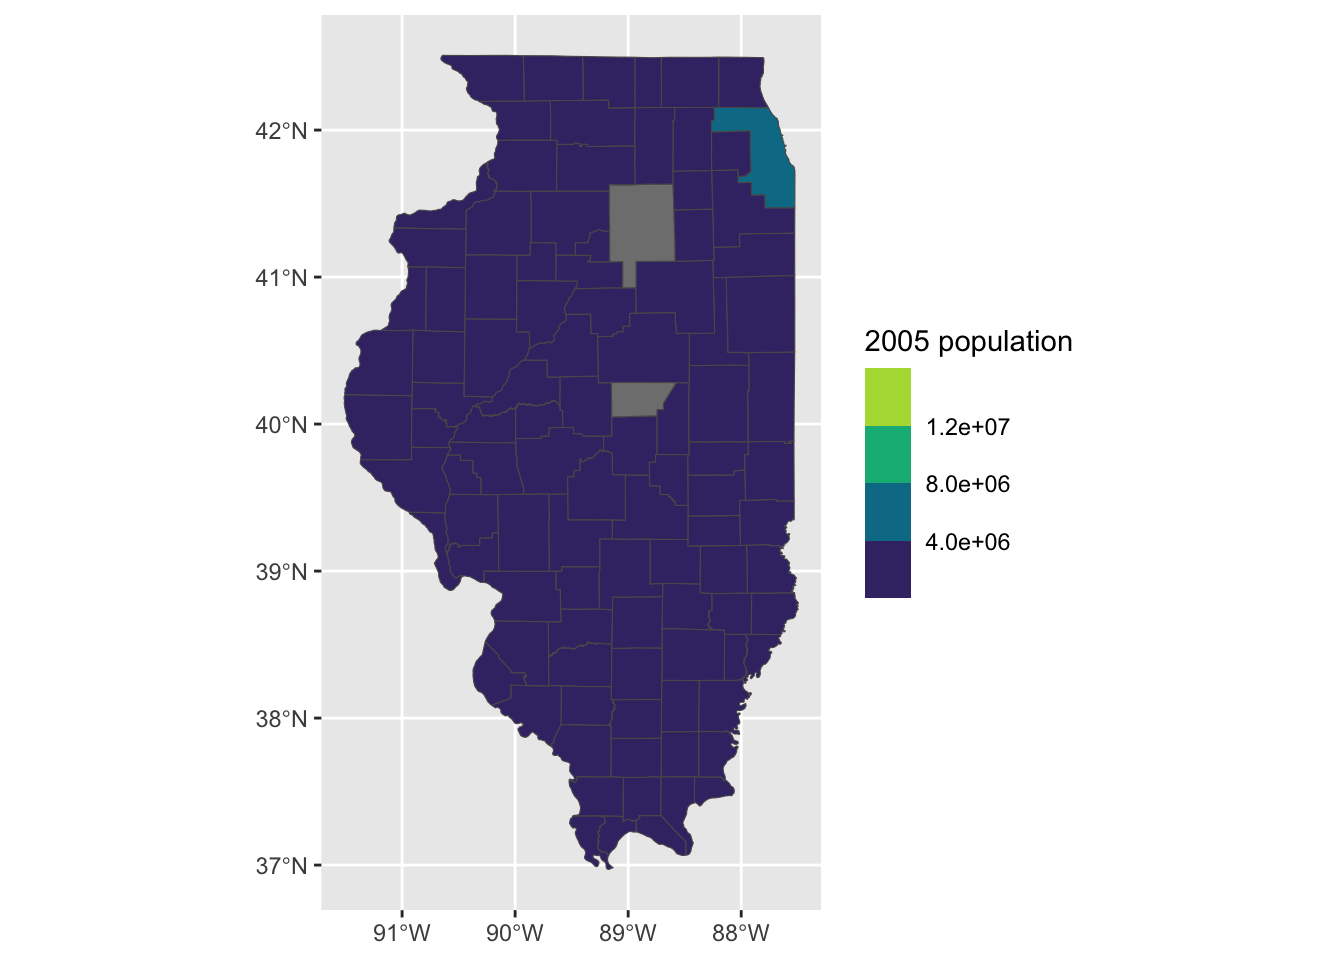
\includegraphics{maps-exercise_files/figure-latex/pop-cut-1.pdf}

\hypertarget{doesnt-look-too-great-lets-try-logging}{%
\subsubsection{Doesn't look too great -- let's try
logging}\label{doesnt-look-too-great-lets-try-logging}}

\begin{Shaded}
\begin{Highlighting}[]
\CommentTok{\#try logging}
\FunctionTok{ggplot}\NormalTok{() }\SpecialCharTok{+} \CommentTok{\# set up basic plot (don\textquotesingle{}t specify data b/c using two data sources)}
 \FunctionTok{geom\_sf}\NormalTok{(}\AttributeTok{data =}\NormalTok{ county\_pop, }\FunctionTok{aes}\NormalTok{(}\AttributeTok{fill =} \StringTok{\textasciigrave{}}\AttributeTok{2005}\StringTok{\textasciigrave{}}\NormalTok{)) }\SpecialCharTok{+} \CommentTok{\# setup our county data}
 \FunctionTok{scale\_fill\_continuous\_sequential}\NormalTok{(}\AttributeTok{palette =} \StringTok{"viridis"}\NormalTok{, }\AttributeTok{rev =} \ConstantTok{FALSE}\NormalTok{, }\AttributeTok{trans =} \StringTok{"log"}\NormalTok{, ) }\SpecialCharTok{+}
  \FunctionTok{labs}\NormalTok{(}\AttributeTok{fill=}\StringTok{"2005 population"}\NormalTok{) }\SpecialCharTok{+} 
  \FunctionTok{coord\_sf}\NormalTok{() }
\end{Highlighting}
\end{Shaded}

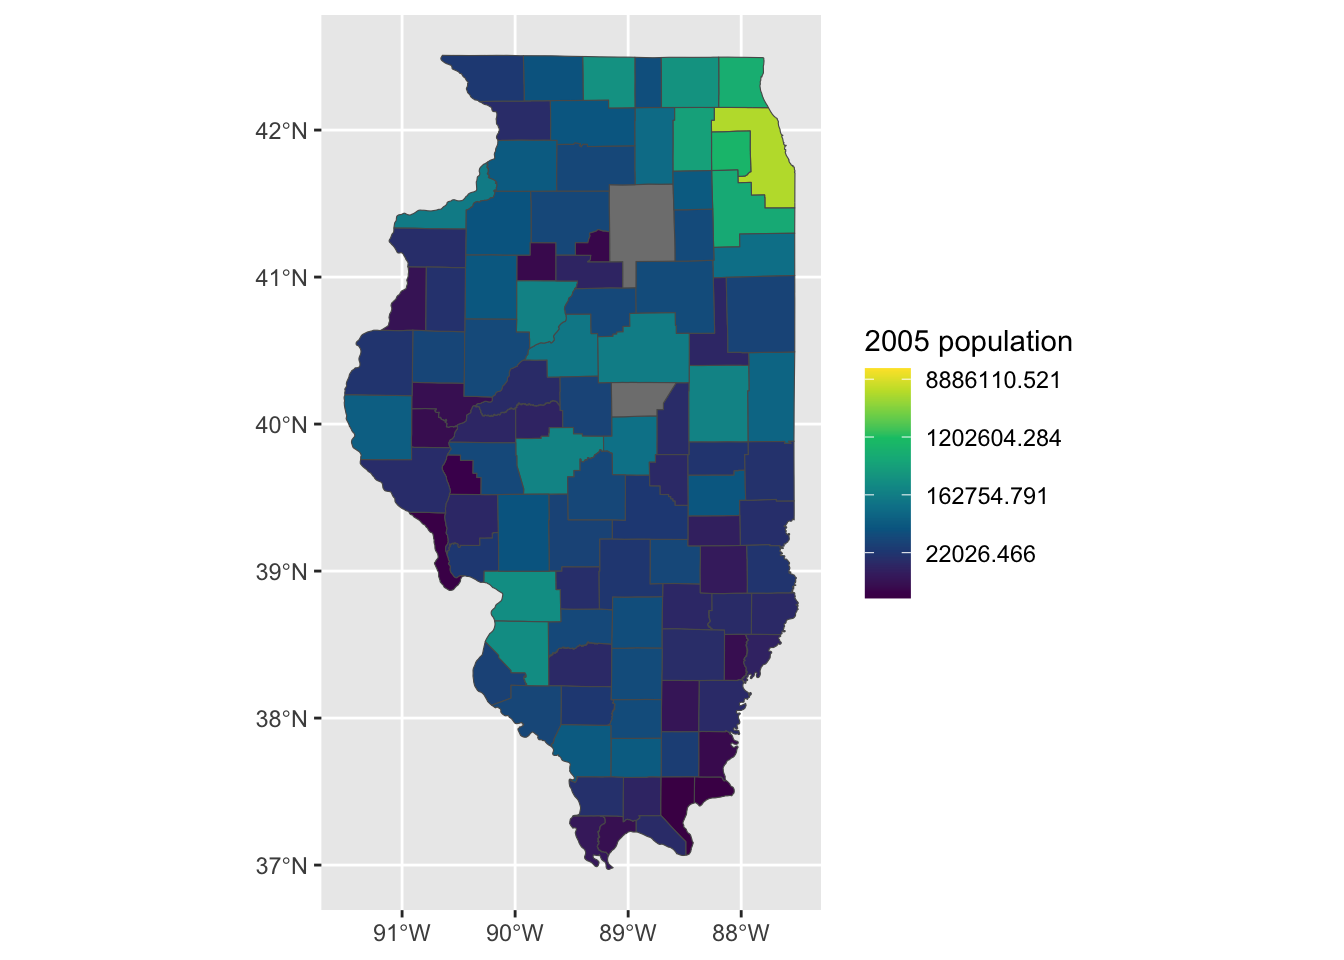
\includegraphics{maps-exercise_files/figure-latex/pop-log-1.pdf}

\begin{Shaded}
\begin{Highlighting}[]
\CommentTok{\# plot}
\FunctionTok{ggplot}\NormalTok{() }\SpecialCharTok{+} \CommentTok{\# set up basic plot (don\textquotesingle{}t specify data b/c using two data sources)}
 \FunctionTok{geom\_sf}\NormalTok{(}\AttributeTok{data =}\NormalTok{ county\_pop, }\FunctionTok{aes}\NormalTok{(}\AttributeTok{fill =} \StringTok{\textasciigrave{}}\AttributeTok{2005}\StringTok{\textasciigrave{}}\NormalTok{)) }\SpecialCharTok{+} \CommentTok{\# setup our county data}
 \FunctionTok{scale\_fill\_continuous\_sequential}\NormalTok{(}\AttributeTok{palette =} \StringTok{"viridis"}\NormalTok{, }\AttributeTok{rev =} \ConstantTok{FALSE}\NormalTok{, }\AttributeTok{trans =} \StringTok{"log"}\NormalTok{, ) }\SpecialCharTok{+}
  \FunctionTok{labs}\NormalTok{(}\AttributeTok{fill=}\StringTok{"2005 population"}\NormalTok{) }\SpecialCharTok{+} 
 \FunctionTok{geom\_point}\NormalTok{(}\AttributeTok{data =}\NormalTok{ illinois,  }\CommentTok{\# bringing in our city data}
            \FunctionTok{aes}\NormalTok{(}\AttributeTok{x =}\NormalTok{ city\_longitude, }\AttributeTok{y =}\NormalTok{ city\_latitude), }
            \AttributeTok{colour =} \StringTok{"white"}\NormalTok{, }\AttributeTok{size =} \FloatTok{0.01}\NormalTok{, }\AttributeTok{alpha =} \FloatTok{0.2}\NormalTok{) }\SpecialCharTok{+} \CommentTok{\# room to improve aesthetically}
  \FunctionTok{coord\_sf}\NormalTok{() }
\end{Highlighting}
\end{Shaded}

\includegraphics{maps-exercise_files/figure-latex/pop-color-1.pdf}

\begin{Shaded}
\begin{Highlighting}[]
\FunctionTok{ggsave}\NormalTok{(}\StringTok{"il\_counties\_cities.png"}\NormalTok{)}
\end{Highlighting}
\end{Shaded}

\begin{verbatim}
## Saving 6.5 x 4.5 in image
\end{verbatim}

\hypertarget{switzerland}{%
\subsection{Switzerland}\label{switzerland}}

\emph{Source:
\url{https://timogrossenbacher.ch/bivariate-maps-with-ggplot2-and-sf/}}
and
\emph{\url{https://timogrossenbacher.ch/bivariate-maps-with-ggplot2-and-sf/}}

\textbf{I did not create any of this, just FYI! it's a streamlined
version from the source website and repo}

\begin{Shaded}
\begin{Highlighting}[]
\CommentTok{\# read cantonal borders}
\NormalTok{canton\_geo }\OtherTok{\textless{}{-}} \FunctionTok{read\_sf}\NormalTok{(}\StringTok{"../data/input/g2k15.shp"}\NormalTok{)}

\CommentTok{\# read country borders}
\NormalTok{country\_geo }\OtherTok{\textless{}{-}} \FunctionTok{read\_sf}\NormalTok{(}\StringTok{"../data/input/g2l15.shp"}\NormalTok{)}

\CommentTok{\# read lakes}
\NormalTok{lake\_geo }\OtherTok{\textless{}{-}} \FunctionTok{read\_sf}\NormalTok{(}\StringTok{"../data/input/g2s15.shp"}\NormalTok{)}

\CommentTok{\# read productive area (2324 municipalities)}
\NormalTok{municipality\_prod\_geo }\OtherTok{\textless{}{-}} \FunctionTok{read\_sf}\NormalTok{(}\StringTok{"../data/input/gde{-}1{-}1{-}15.shp"}\NormalTok{)}

\CommentTok{\# read in raster of relief}
\NormalTok{relief }\OtherTok{\textless{}{-}} \FunctionTok{raster}\NormalTok{(}\StringTok{"../data/input/02{-}relief{-}ascii.asc"}\NormalTok{) }\SpecialCharTok{\%\textgreater{}\%}
  \CommentTok{\# hide relief outside of Switzerland by masking with country borders}
  \FunctionTok{mask}\NormalTok{(country\_geo) }\SpecialCharTok{\%\textgreater{}\%}
  \FunctionTok{as}\NormalTok{(}\StringTok{"SpatialPixelsDataFrame"}\NormalTok{) }\SpecialCharTok{\%\textgreater{}\%}
  \FunctionTok{as.data.frame}\NormalTok{() }\SpecialCharTok{\%\textgreater{}\%}
  \FunctionTok{rename}\NormalTok{(}\AttributeTok{value =} \StringTok{\textasciigrave{}}\AttributeTok{X02.relief.ascii}\StringTok{\textasciigrave{}}\NormalTok{)}

\CommentTok{\# clean up}
\FunctionTok{rm}\NormalTok{(country\_geo)}
\end{Highlighting}
\end{Shaded}

\begin{Shaded}
\begin{Highlighting}[]
\NormalTok{data }\OtherTok{\textless{}{-}} \FunctionTok{read\_csv}\NormalTok{(}\StringTok{"../data/input/data.csv"}\NormalTok{)}

\CommentTok{\# create 3 buckets for gini}
\NormalTok{quantiles\_gini }\OtherTok{\textless{}{-}}\NormalTok{ data }\SpecialCharTok{\%\textgreater{}\%}
  \FunctionTok{pull}\NormalTok{(gini) }\SpecialCharTok{\%\textgreater{}\%}
  \FunctionTok{quantile}\NormalTok{(}\AttributeTok{probs =} \FunctionTok{seq}\NormalTok{(}\DecValTok{0}\NormalTok{, }\DecValTok{1}\NormalTok{, }\AttributeTok{length.out =} \DecValTok{4}\NormalTok{))}

\CommentTok{\# create 3 buckets for mean income}
\NormalTok{quantiles\_mean }\OtherTok{\textless{}{-}}\NormalTok{ data }\SpecialCharTok{\%\textgreater{}\%}
  \FunctionTok{pull}\NormalTok{(mean) }\SpecialCharTok{\%\textgreater{}\%}
  \FunctionTok{quantile}\NormalTok{(}\AttributeTok{probs =} \FunctionTok{seq}\NormalTok{(}\DecValTok{0}\NormalTok{, }\DecValTok{1}\NormalTok{, }\AttributeTok{length.out =} \DecValTok{4}\NormalTok{))}

\CommentTok{\# create color scale that encodes two variables}
\CommentTok{\# red for gini and blue for mean income}
\CommentTok{\# the special notation with gather is due to readibility reasons}
\NormalTok{bivariate\_color\_scale }\OtherTok{\textless{}{-}} \FunctionTok{tibble}\NormalTok{(}
  \StringTok{"3 {-} 3"} \OtherTok{=} \StringTok{"\#3F2949"}\NormalTok{, }\CommentTok{\# high inequality, high income}
  \StringTok{"2 {-} 3"} \OtherTok{=} \StringTok{"\#435786"}\NormalTok{,}
  \StringTok{"1 {-} 3"} \OtherTok{=} \StringTok{"\#4885C1"}\NormalTok{, }\CommentTok{\# low inequality, high income}
  \StringTok{"3 {-} 2"} \OtherTok{=} \StringTok{"\#77324C"}\NormalTok{,}
  \StringTok{"2 {-} 2"} \OtherTok{=} \StringTok{"\#806A8A"}\NormalTok{, }\CommentTok{\# medium inequality, medium income}
  \StringTok{"1 {-} 2"} \OtherTok{=} \StringTok{"\#89A1C8"}\NormalTok{,}
  \StringTok{"3 {-} 1"} \OtherTok{=} \StringTok{"\#AE3A4E"}\NormalTok{, }\CommentTok{\# high inequality, low income}
  \StringTok{"2 {-} 1"} \OtherTok{=} \StringTok{"\#BC7C8F"}\NormalTok{,}
  \StringTok{"1 {-} 1"} \OtherTok{=} \StringTok{"\#CABED0"} \CommentTok{\# low inequality, low income}
\NormalTok{) }\SpecialCharTok{\%\textgreater{}\%}
  \FunctionTok{gather}\NormalTok{(}\StringTok{"group"}\NormalTok{, }\StringTok{"fill"}\NormalTok{)}
\end{Highlighting}
\end{Shaded}

\hypertarget{join-color-codes-to-the-data}{%
\subsubsection{Join Color Codes to the
Data}\label{join-color-codes-to-the-data}}

Here the municipalities are put into the appropriate class corresponding
to their average income and income (in-)equality.

\begin{Shaded}
\begin{Highlighting}[]
\CommentTok{\# cut into groups defined above and join fill}
\NormalTok{municipality\_prod\_geo }\OtherTok{\textless{}{-}}\NormalTok{ municipality\_prod\_geo }\SpecialCharTok{\%\textgreater{}\%}
  \FunctionTok{left\_join}\NormalTok{(data, }\AttributeTok{by =} \FunctionTok{c}\NormalTok{(}\StringTok{"BFS\_ID"} \OtherTok{=} \StringTok{"bfs\_id"}\NormalTok{))}
\FunctionTok{class}\NormalTok{(municipality\_prod\_geo)}
\end{Highlighting}
\end{Shaded}

\begin{verbatim}
## [1] "sf"         "tbl_df"     "tbl"        "data.frame"
\end{verbatim}

\begin{Shaded}
\begin{Highlighting}[]
\NormalTok{municipality\_prod\_geo }\OtherTok{\textless{}{-}}\NormalTok{ municipality\_prod\_geo }\SpecialCharTok{\%\textgreater{}\%}
  \FunctionTok{mutate}\NormalTok{(}
    \AttributeTok{gini\_quantiles =} \FunctionTok{cut}\NormalTok{(}
\NormalTok{      gini,}
      \AttributeTok{breaks =}\NormalTok{ quantiles\_gini,}
      \AttributeTok{include.lowest =} \ConstantTok{TRUE}
\NormalTok{    ),}
    \AttributeTok{mean\_quantiles =} \FunctionTok{cut}\NormalTok{(}
\NormalTok{      mean,}
      \AttributeTok{breaks =}\NormalTok{ quantiles\_mean,}
      \AttributeTok{include.lowest =} \ConstantTok{TRUE}
\NormalTok{    ),}
    \CommentTok{\# by pasting the factors together as numbers we match the groups defined}
    \CommentTok{\# in the tibble bivariate\_color\_scale}
    \AttributeTok{group =} \FunctionTok{paste}\NormalTok{(}
      \FunctionTok{as.numeric}\NormalTok{(gini\_quantiles), }\StringTok{"{-}"}\NormalTok{,}
      \FunctionTok{as.numeric}\NormalTok{(mean\_quantiles)}
\NormalTok{    )}
\NormalTok{  ) }\SpecialCharTok{\%\textgreater{}\%}
  \CommentTok{\# we now join the actual hex values per "group"}
  \CommentTok{\# so each municipality knows its hex value based on the his gini and avg}
  \CommentTok{\# income value}
  \FunctionTok{left\_join}\NormalTok{(bivariate\_color\_scale, }\AttributeTok{by =} \StringTok{"group"}\NormalTok{)}
\end{Highlighting}
\end{Shaded}

\begin{Shaded}
\begin{Highlighting}[]
\FunctionTok{ggplot}\NormalTok{(}
  \CommentTok{\# define main data source}
  \AttributeTok{data =}\NormalTok{ municipality\_prod\_geo}
\NormalTok{) }\SpecialCharTok{+}
    \CommentTok{\# raster comes as the first layer, municipalities on top}
    \FunctionTok{geom\_raster}\NormalTok{(}
      \AttributeTok{data =}\NormalTok{ relief, }\FunctionTok{aes}\NormalTok{( }\AttributeTok{x =}\NormalTok{ x,   }\AttributeTok{y =}\NormalTok{ y,  }\AttributeTok{alpha =}\NormalTok{ value  ) ) }\SpecialCharTok{+}
    \CommentTok{\# use the "alpha hack"}
    \FunctionTok{scale\_alpha}\NormalTok{(}\AttributeTok{name =} \StringTok{""}\NormalTok{, }\AttributeTok{range =} \FunctionTok{c}\NormalTok{(}\FloatTok{0.6}\NormalTok{, }\DecValTok{0}\NormalTok{), }\AttributeTok{guide =} \ConstantTok{FALSE}\NormalTok{)  }\SpecialCharTok{+} 
  \FunctionTok{geom\_sf}\NormalTok{(}
    \AttributeTok{mapping =} \FunctionTok{aes}\NormalTok{(}
      \AttributeTok{fill =}\NormalTok{ fill}
\NormalTok{      ),}
    \AttributeTok{color =} \StringTok{"white"}\NormalTok{,}
    \AttributeTok{size =} \FloatTok{0.1}
\NormalTok{  ) }\SpecialCharTok{+}
  \CommentTok{\# use the Viridis color scale}
  \FunctionTok{scale\_fill\_viridis}\NormalTok{(}
    \AttributeTok{option =} \StringTok{"magma"}\NormalTok{,}
    \AttributeTok{name =} \StringTok{"Average}\SpecialCharTok{\textbackslash{}n}\StringTok{income in CHF"}\NormalTok{,}
    \AttributeTok{alpha =} \FloatTok{0.8}\NormalTok{, }\CommentTok{\# make fill a bit brighter}
    \AttributeTok{begin =} \FloatTok{0.1}\NormalTok{, }\CommentTok{\# this option seems to be new (compared to 2016):}
    \CommentTok{\# with this we can truncate the}
    \CommentTok{\# color scale, so that extreme colors (very dark and very bright) are not}
    \CommentTok{\# used, which makes the map a bit more aesthetic}
    \AttributeTok{end =} \FloatTok{0.9}\NormalTok{,}
    \AttributeTok{discrete =}\NormalTok{ T, }\CommentTok{\# discrete classes, thus guide\_legend instead of \_colorbar}
    \AttributeTok{direction =} \DecValTok{1}\NormalTok{, }\CommentTok{\# dark is lowest, yellow is highest}
    \AttributeTok{guide =} \FunctionTok{guide\_legend}\NormalTok{(}
     \AttributeTok{keyheight =} \FunctionTok{unit}\NormalTok{(}\DecValTok{5}\NormalTok{, }\AttributeTok{units =} \StringTok{"mm"}\NormalTok{),}
     \AttributeTok{title.position =} \StringTok{"top"}\NormalTok{,}
     \AttributeTok{reverse =}\NormalTok{ T }\CommentTok{\# display highest income on top}
\NormalTok{  )) }\SpecialCharTok{+}
  \FunctionTok{geom\_sf}\NormalTok{(}
    \AttributeTok{data =}\NormalTok{ canton\_geo,}
    \AttributeTok{fill =} \StringTok{"transparent"}\NormalTok{,}
    \AttributeTok{color =} \StringTok{"white"}\NormalTok{,}
    \AttributeTok{size =} \FloatTok{0.5}
\NormalTok{  )}\SpecialCharTok{+}
  \CommentTok{\# draw lakes in light blue}
  \FunctionTok{geom\_sf}\NormalTok{(}
    \AttributeTok{data =}\NormalTok{ lake\_geo,}
    \AttributeTok{fill =} \StringTok{"\#D6F1FF"}\NormalTok{,}
    \AttributeTok{color =} \StringTok{"transparent"}
\NormalTok{  ) }\SpecialCharTok{+}
  \CommentTok{\# add titles}
  \FunctionTok{labs}\NormalTok{(}\AttributeTok{x =} \ConstantTok{NULL}\NormalTok{,}
         \AttributeTok{y =} \ConstantTok{NULL}\NormalTok{,}
         \AttributeTok{title =} \StringTok{"Switzerland\textquotesingle{}s regional income (in{-})equality"}\NormalTok{,}
         \AttributeTok{subtitle =} \FunctionTok{paste0}\NormalTok{(}\StringTok{"Average yearly income and income"}\NormalTok{,}
                           \StringTok{" (in{-})equality in Swiss municipalities, 2015"}\NormalTok{))}
\end{Highlighting}
\end{Shaded}

\begin{verbatim}
## Warning: The `guide` argument in `scale_*()` cannot be `FALSE`. This was deprecated in
## ggplot2 3.3.4.
## i Please use "none" instead.
## This warning is displayed once every 8 hours.
## Call `lifecycle::last_lifecycle_warnings()` to see where this warning was
## generated.
\end{verbatim}

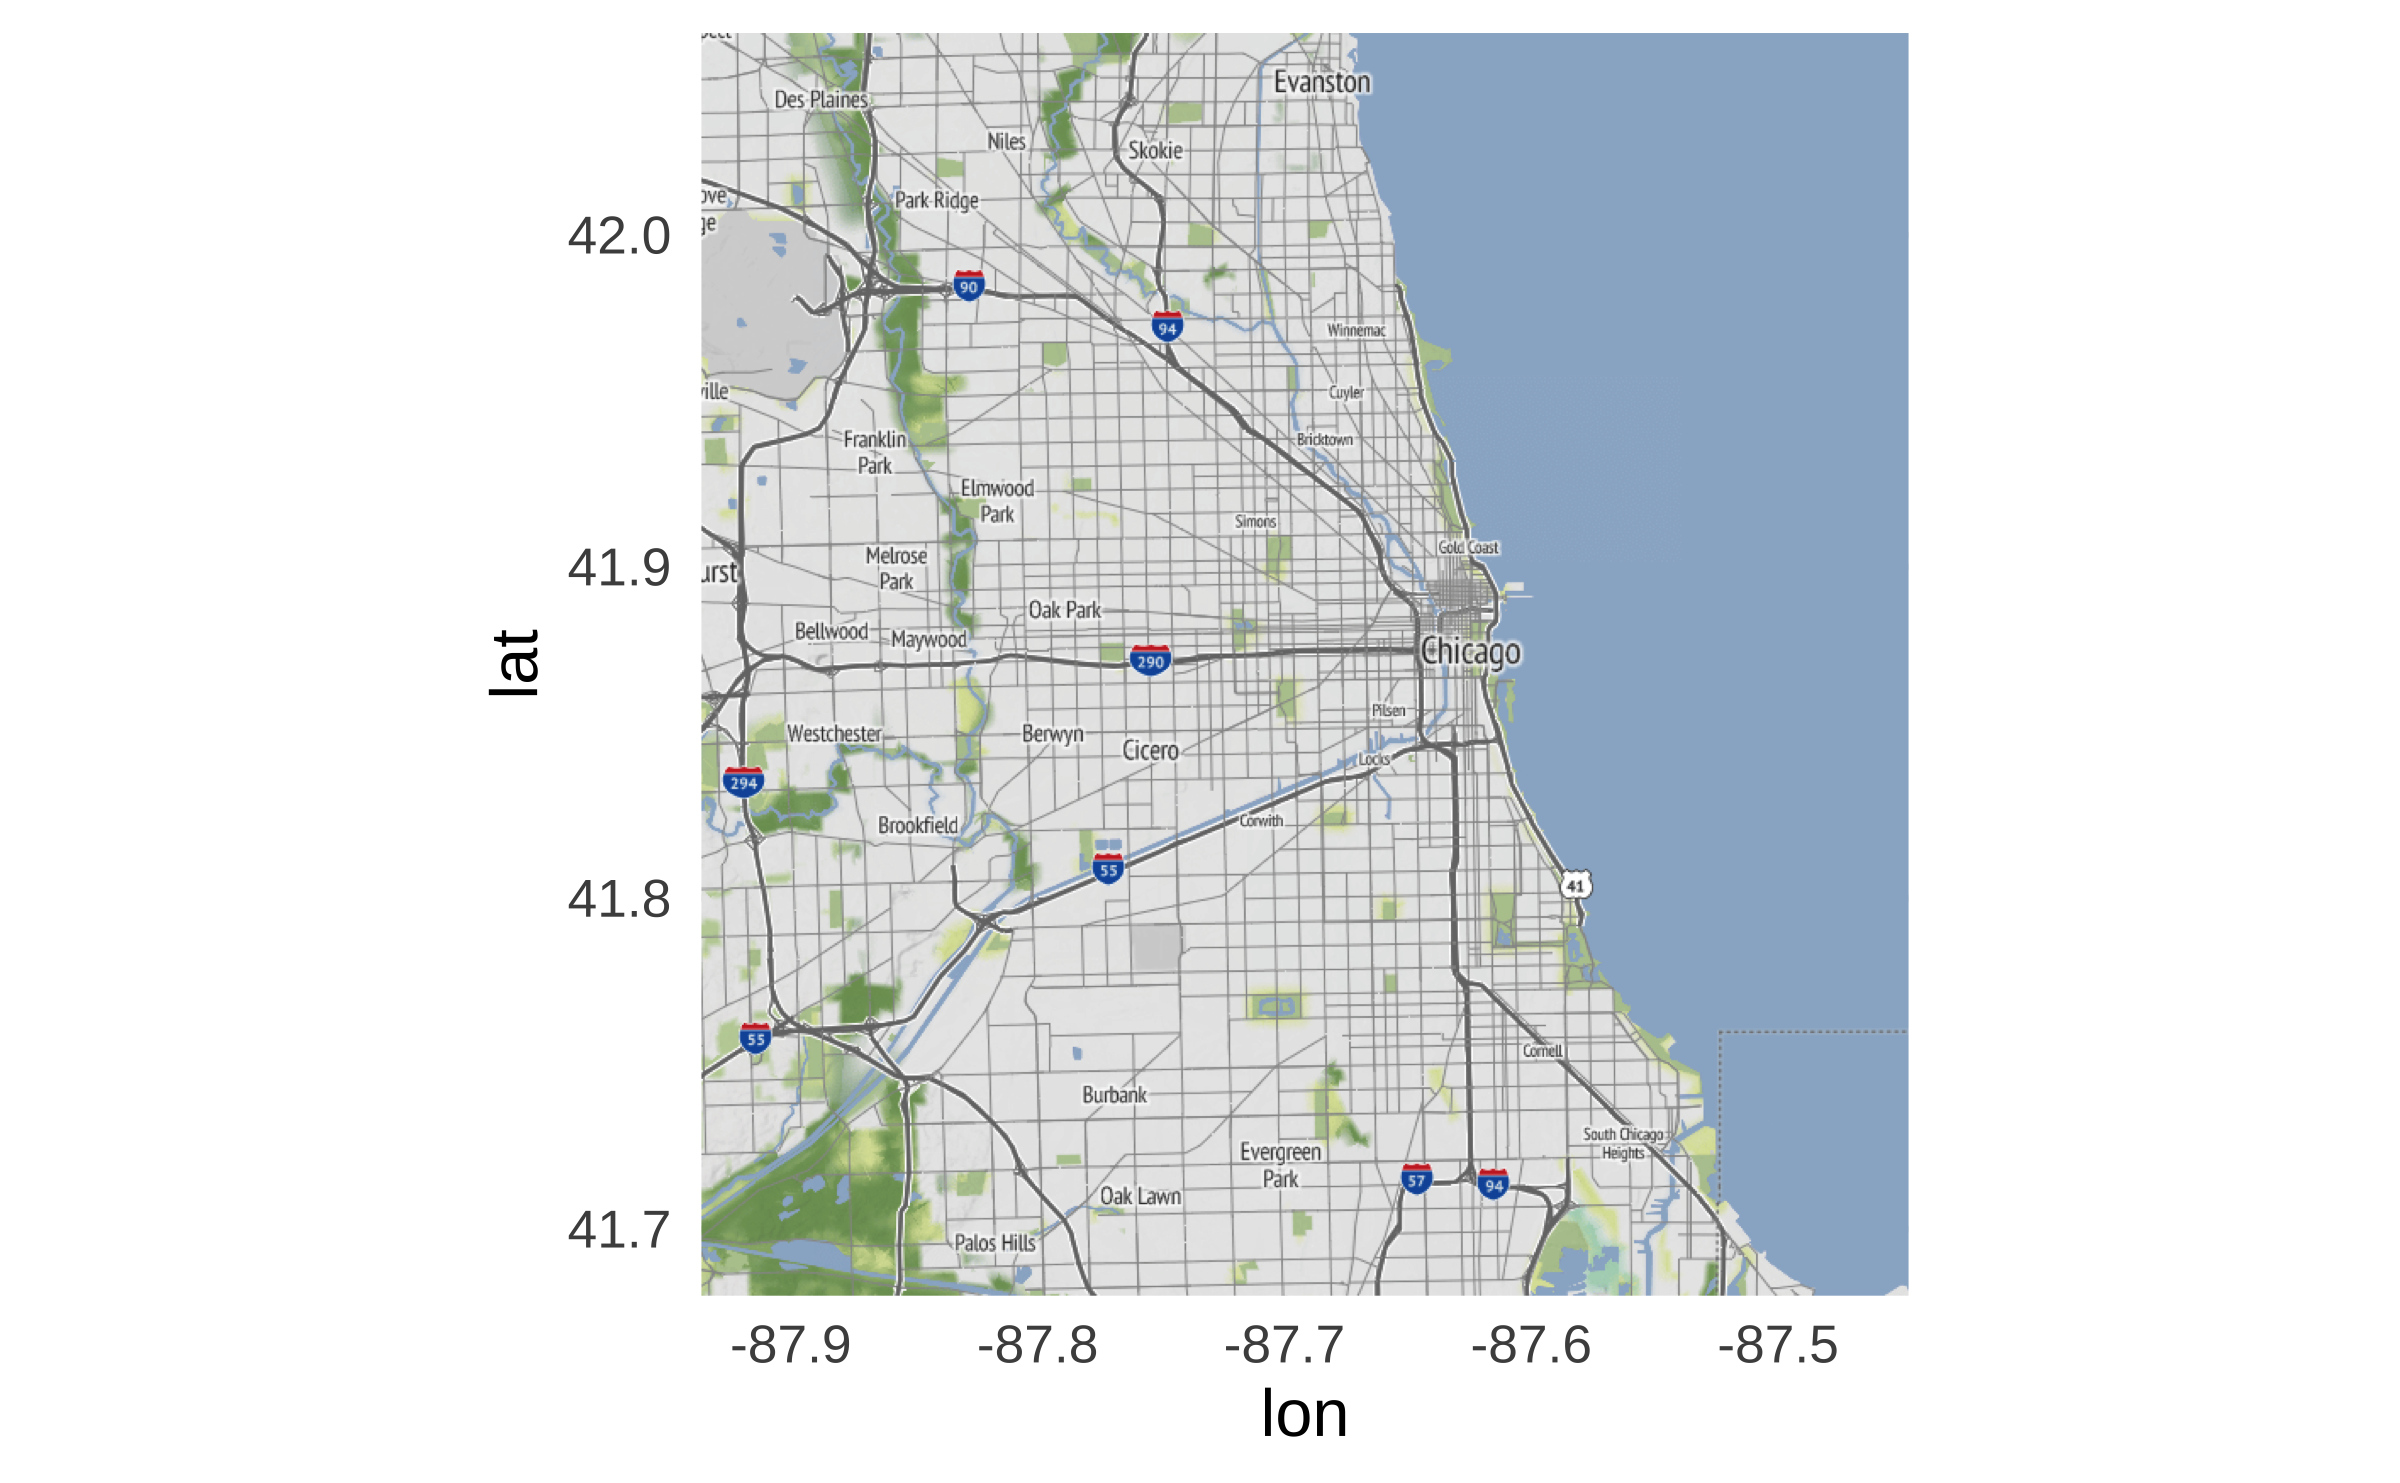
\includegraphics{maps-exercise_files/figure-latex/unnamed-chunk-6-1.pdf}

\hypertarget{making-it-fancy}{%
\subsubsection{\texorpdfstring{Making it
\textsubscript{fancy}}{Making it fancy}}\label{making-it-fancy}}

\begin{Shaded}
\begin{Highlighting}[]
\NormalTok{map }\OtherTok{\textless{}{-}} \FunctionTok{ggplot}\NormalTok{(}
  \CommentTok{\# use the same dataset as before}
  \AttributeTok{data =}\NormalTok{ municipality\_prod\_geo}
\NormalTok{  ) }\SpecialCharTok{+}
  \CommentTok{\# first: draw the relief}
  \FunctionTok{geom\_raster}\NormalTok{(}
    \AttributeTok{data =}\NormalTok{ relief,}
    \FunctionTok{aes}\NormalTok{(}
      \AttributeTok{x =}\NormalTok{ x,}
      \AttributeTok{y =}\NormalTok{ y,}
      \AttributeTok{alpha =}\NormalTok{ value}
\NormalTok{    )}
\NormalTok{  ) }\SpecialCharTok{+}
  \CommentTok{\# use the "alpha hack" (as the "fill" aesthetic is already taken)}
  \FunctionTok{scale\_alpha}\NormalTok{(}\AttributeTok{name =} \StringTok{""}\NormalTok{,}
              \AttributeTok{range =} \FunctionTok{c}\NormalTok{(}\FloatTok{0.6}\NormalTok{, }\DecValTok{0}\NormalTok{),}
              \AttributeTok{guide =}\NormalTok{ F) }\SpecialCharTok{+} \CommentTok{\# suppress legend}
  \CommentTok{\# color municipalities according to their gini / income combination}
  \FunctionTok{geom\_sf}\NormalTok{(}
    \FunctionTok{aes}\NormalTok{(}
      \AttributeTok{fill =}\NormalTok{ fill}
\NormalTok{    ),}
    \CommentTok{\# use thin white stroke for municipalities}
    \AttributeTok{color =} \StringTok{"white"}\NormalTok{,}
    \AttributeTok{size =} \FloatTok{0.1}
\NormalTok{  ) }\SpecialCharTok{+}
  \CommentTok{\# as the sf object municipality\_prod\_geo has a column with name "fill" that}
  \CommentTok{\# contains the literal color as hex code for each municipality, we can use}
  \CommentTok{\# scale\_fill\_identity here}
  \FunctionTok{scale\_fill\_identity}\NormalTok{() }\SpecialCharTok{+}
  \CommentTok{\# use thicker white stroke for cantons}
  \FunctionTok{geom\_sf}\NormalTok{(}
    \AttributeTok{data =}\NormalTok{ canton\_geo,}
    \AttributeTok{fill =} \StringTok{"transparent"}\NormalTok{,}
    \AttributeTok{color =} \StringTok{"white"}\NormalTok{,}
    \AttributeTok{size =} \FloatTok{0.5}
\NormalTok{  ) }\SpecialCharTok{+}
  \CommentTok{\# draw lakes in light blue}
  \FunctionTok{geom\_sf}\NormalTok{(}
    \AttributeTok{data =}\NormalTok{ lake\_geo,}
    \AttributeTok{fill =} \StringTok{"\#D6F1FF"}\NormalTok{,}
    \AttributeTok{color =} \StringTok{"transparent"}
\NormalTok{  ) }\SpecialCharTok{+}
  \CommentTok{\# add titles}
  \FunctionTok{labs}\NormalTok{(}\AttributeTok{x =} \ConstantTok{NULL}\NormalTok{,}
         \AttributeTok{y =} \ConstantTok{NULL}\NormalTok{,}
         \AttributeTok{title =} \StringTok{"Switzerland\textquotesingle{}s regional income (in{-})equality"}\NormalTok{,}
         \AttributeTok{subtitle =} \FunctionTok{paste0}\NormalTok{(}\StringTok{"Average yearly income and income"}\NormalTok{,}
                           \StringTok{" (in{-})equality in Swiss municipalities, 2015"}\NormalTok{)) }\SpecialCharTok{+}
  \CommentTok{\# add the theme}
  \FunctionTok{theme\_map}\NormalTok{()}
\end{Highlighting}
\end{Shaded}

\begin{Shaded}
\begin{Highlighting}[]
\CommentTok{\# separate the groups}
\NormalTok{bivariate\_color\_scale }\OtherTok{\textless{}{-}}\NormalTok{ bivariate\_color\_scale }\SpecialCharTok{\%\textgreater{}\%}
  \FunctionTok{separate}\NormalTok{(group, }\AttributeTok{into =} \FunctionTok{c}\NormalTok{(}\StringTok{"gini"}\NormalTok{, }\StringTok{"mean"}\NormalTok{), }\AttributeTok{sep =} \StringTok{" {-} "}\NormalTok{) }\SpecialCharTok{\%\textgreater{}\%}
  \FunctionTok{mutate}\NormalTok{(}\AttributeTok{gini =} \FunctionTok{as.integer}\NormalTok{(gini),}
         \AttributeTok{mean =} \FunctionTok{as.integer}\NormalTok{(mean))}

\NormalTok{legend }\OtherTok{\textless{}{-}} \FunctionTok{ggplot}\NormalTok{() }\SpecialCharTok{+}
  \FunctionTok{geom\_tile}\NormalTok{(}
    \AttributeTok{data =}\NormalTok{ bivariate\_color\_scale,}
    \AttributeTok{mapping =} \FunctionTok{aes}\NormalTok{(}
      \AttributeTok{x =}\NormalTok{ gini,}
      \AttributeTok{y =}\NormalTok{ mean,}
      \AttributeTok{fill =}\NormalTok{ fill)}
\NormalTok{  ) }\SpecialCharTok{+}
  \FunctionTok{scale\_fill\_identity}\NormalTok{() }\SpecialCharTok{+}
  \FunctionTok{labs}\NormalTok{(}\AttributeTok{x =} \StringTok{"Higher inequality ⟶️"}\NormalTok{,}
       \AttributeTok{y =} \StringTok{"Higher income ⟶️"}\NormalTok{) }\SpecialCharTok{+}
  \FunctionTok{theme\_map}\NormalTok{() }\SpecialCharTok{+}
  \CommentTok{\# make font small enough}
  \FunctionTok{theme}\NormalTok{(}
    \AttributeTok{axis.title =} \FunctionTok{element\_text}\NormalTok{(}\AttributeTok{size =} \DecValTok{6}\NormalTok{)}
\NormalTok{  ) }\SpecialCharTok{+}
  \CommentTok{\# quadratic tiles}
  \FunctionTok{coord\_fixed}\NormalTok{()}
\end{Highlighting}
\end{Shaded}

\begin{Shaded}
\begin{Highlighting}[]
\FunctionTok{ggdraw}\NormalTok{() }\SpecialCharTok{+}
  \FunctionTok{draw\_plot}\NormalTok{(map, }\DecValTok{0}\NormalTok{, }\DecValTok{0}\NormalTok{, }\DecValTok{1}\NormalTok{, }\DecValTok{1}\NormalTok{) }\SpecialCharTok{+}
  \FunctionTok{draw\_plot}\NormalTok{(legend, }\FloatTok{0.05}\NormalTok{, }\FloatTok{0.075}\NormalTok{, }\FloatTok{0.2}\NormalTok{, }\FloatTok{0.2}\NormalTok{)}
\end{Highlighting}
\end{Shaded}

\begin{verbatim}
## Warning in grid.Call(C_textBounds, as.graphicsAnnot(x$label), x$x, x$y, :
## conversion failure on 'Higher income ⟶️' in 'mbcsToSbcs': dot substituted for
## <e2>
\end{verbatim}

\begin{verbatim}
## Warning in grid.Call(C_textBounds, as.graphicsAnnot(x$label), x$x, x$y, :
## conversion failure on 'Higher income ⟶️' in 'mbcsToSbcs': dot substituted for
## <9f>
\end{verbatim}

\begin{verbatim}
## Warning in grid.Call(C_textBounds, as.graphicsAnnot(x$label), x$x, x$y, :
## conversion failure on 'Higher income ⟶️' in 'mbcsToSbcs': dot substituted for
## <b6>
\end{verbatim}

\begin{verbatim}
## Warning in grid.Call(C_textBounds, as.graphicsAnnot(x$label), x$x, x$y, :
## conversion failure on 'Higher income ⟶️' in 'mbcsToSbcs': dot substituted for
## <ef>
\end{verbatim}

\begin{verbatim}
## Warning in grid.Call(C_textBounds, as.graphicsAnnot(x$label), x$x, x$y, :
## conversion failure on 'Higher income ⟶️' in 'mbcsToSbcs': dot substituted for
## <b8>
\end{verbatim}

\begin{verbatim}
## Warning in grid.Call(C_textBounds, as.graphicsAnnot(x$label), x$x, x$y, :
## conversion failure on 'Higher income ⟶️' in 'mbcsToSbcs': dot substituted for
## <8f>
\end{verbatim}

\begin{verbatim}
## Warning in grid.Call(C_textBounds, as.graphicsAnnot(x$label), x$x, x$y, :
## conversion failure on 'Higher income ⟶️' in 'mbcsToSbcs': dot substituted for
## <e2>
\end{verbatim}

\begin{verbatim}
## Warning in grid.Call(C_textBounds, as.graphicsAnnot(x$label), x$x, x$y, :
## conversion failure on 'Higher income ⟶️' in 'mbcsToSbcs': dot substituted for
## <9f>
\end{verbatim}

\begin{verbatim}
## Warning in grid.Call(C_textBounds, as.graphicsAnnot(x$label), x$x, x$y, :
## conversion failure on 'Higher income ⟶️' in 'mbcsToSbcs': dot substituted for
## <b6>
\end{verbatim}

\begin{verbatim}
## Warning in grid.Call(C_textBounds, as.graphicsAnnot(x$label), x$x, x$y, :
## conversion failure on 'Higher income ⟶️' in 'mbcsToSbcs': dot substituted for
## <ef>
\end{verbatim}

\begin{verbatim}
## Warning in grid.Call(C_textBounds, as.graphicsAnnot(x$label), x$x, x$y, :
## conversion failure on 'Higher income ⟶️' in 'mbcsToSbcs': dot substituted for
## <b8>
\end{verbatim}

\begin{verbatim}
## Warning in grid.Call(C_textBounds, as.graphicsAnnot(x$label), x$x, x$y, :
## conversion failure on 'Higher income ⟶️' in 'mbcsToSbcs': dot substituted for
## <8f>
\end{verbatim}

\begin{verbatim}
## Warning in grid.Call(C_textBounds, as.graphicsAnnot(x$label), x$x, x$y, :
## conversion failure on 'Higher inequality ⟶️' in 'mbcsToSbcs': dot substituted
## for <e2>
\end{verbatim}

\begin{verbatim}
## Warning in grid.Call(C_textBounds, as.graphicsAnnot(x$label), x$x, x$y, :
## conversion failure on 'Higher inequality ⟶️' in 'mbcsToSbcs': dot substituted
## for <9f>
\end{verbatim}

\begin{verbatim}
## Warning in grid.Call(C_textBounds, as.graphicsAnnot(x$label), x$x, x$y, :
## conversion failure on 'Higher inequality ⟶️' in 'mbcsToSbcs': dot substituted
## for <b6>
\end{verbatim}

\begin{verbatim}
## Warning in grid.Call(C_textBounds, as.graphicsAnnot(x$label), x$x, x$y, :
## conversion failure on 'Higher inequality ⟶️' in 'mbcsToSbcs': dot substituted
## for <ef>
\end{verbatim}

\begin{verbatim}
## Warning in grid.Call(C_textBounds, as.graphicsAnnot(x$label), x$x, x$y, :
## conversion failure on 'Higher inequality ⟶️' in 'mbcsToSbcs': dot substituted
## for <b8>
\end{verbatim}

\begin{verbatim}
## Warning in grid.Call(C_textBounds, as.graphicsAnnot(x$label), x$x, x$y, :
## conversion failure on 'Higher inequality ⟶️' in 'mbcsToSbcs': dot substituted
## for <8f>
\end{verbatim}

\begin{verbatim}
## Warning in grid.Call(C_textBounds, as.graphicsAnnot(x$label), x$x, x$y, :
## conversion failure on 'Higher inequality ⟶️' in 'mbcsToSbcs': dot substituted
## for <e2>
\end{verbatim}

\begin{verbatim}
## Warning in grid.Call(C_textBounds, as.graphicsAnnot(x$label), x$x, x$y, :
## conversion failure on 'Higher inequality ⟶️' in 'mbcsToSbcs': dot substituted
## for <9f>
\end{verbatim}

\begin{verbatim}
## Warning in grid.Call(C_textBounds, as.graphicsAnnot(x$label), x$x, x$y, :
## conversion failure on 'Higher inequality ⟶️' in 'mbcsToSbcs': dot substituted
## for <b6>
\end{verbatim}

\begin{verbatim}
## Warning in grid.Call(C_textBounds, as.graphicsAnnot(x$label), x$x, x$y, :
## conversion failure on 'Higher inequality ⟶️' in 'mbcsToSbcs': dot substituted
## for <ef>
\end{verbatim}

\begin{verbatim}
## Warning in grid.Call(C_textBounds, as.graphicsAnnot(x$label), x$x, x$y, :
## conversion failure on 'Higher inequality ⟶️' in 'mbcsToSbcs': dot substituted
## for <b8>
\end{verbatim}

\begin{verbatim}
## Warning in grid.Call(C_textBounds, as.graphicsAnnot(x$label), x$x, x$y, :
## conversion failure on 'Higher inequality ⟶️' in 'mbcsToSbcs': dot substituted
## for <8f>
\end{verbatim}

\begin{verbatim}
## Warning in grid.Call(C_textBounds, as.graphicsAnnot(x$label), x$x, x$y, :
## conversion failure on 'Higher income ⟶️' in 'mbcsToSbcs': dot substituted for
## <e2>
\end{verbatim}

\begin{verbatim}
## Warning in grid.Call(C_textBounds, as.graphicsAnnot(x$label), x$x, x$y, :
## conversion failure on 'Higher income ⟶️' in 'mbcsToSbcs': dot substituted for
## <9f>
\end{verbatim}

\begin{verbatim}
## Warning in grid.Call(C_textBounds, as.graphicsAnnot(x$label), x$x, x$y, :
## conversion failure on 'Higher income ⟶️' in 'mbcsToSbcs': dot substituted for
## <b6>
\end{verbatim}

\begin{verbatim}
## Warning in grid.Call(C_textBounds, as.graphicsAnnot(x$label), x$x, x$y, :
## conversion failure on 'Higher income ⟶️' in 'mbcsToSbcs': dot substituted for
## <ef>
\end{verbatim}

\begin{verbatim}
## Warning in grid.Call(C_textBounds, as.graphicsAnnot(x$label), x$x, x$y, :
## conversion failure on 'Higher income ⟶️' in 'mbcsToSbcs': dot substituted for
## <b8>
\end{verbatim}

\begin{verbatim}
## Warning in grid.Call(C_textBounds, as.graphicsAnnot(x$label), x$x, x$y, :
## conversion failure on 'Higher income ⟶️' in 'mbcsToSbcs': dot substituted for
## <8f>
\end{verbatim}

\begin{verbatim}
## Warning in grid.Call(C_textBounds, as.graphicsAnnot(x$label), x$x, x$y, :
## conversion failure on 'Higher income ⟶️' in 'mbcsToSbcs': dot substituted for
## <e2>
\end{verbatim}

\begin{verbatim}
## Warning in grid.Call(C_textBounds, as.graphicsAnnot(x$label), x$x, x$y, :
## conversion failure on 'Higher income ⟶️' in 'mbcsToSbcs': dot substituted for
## <9f>
\end{verbatim}

\begin{verbatim}
## Warning in grid.Call(C_textBounds, as.graphicsAnnot(x$label), x$x, x$y, :
## conversion failure on 'Higher income ⟶️' in 'mbcsToSbcs': dot substituted for
## <b6>
\end{verbatim}

\begin{verbatim}
## Warning in grid.Call(C_textBounds, as.graphicsAnnot(x$label), x$x, x$y, :
## conversion failure on 'Higher income ⟶️' in 'mbcsToSbcs': dot substituted for
## <ef>
\end{verbatim}

\begin{verbatim}
## Warning in grid.Call(C_textBounds, as.graphicsAnnot(x$label), x$x, x$y, :
## conversion failure on 'Higher income ⟶️' in 'mbcsToSbcs': dot substituted for
## <b8>
\end{verbatim}

\begin{verbatim}
## Warning in grid.Call(C_textBounds, as.graphicsAnnot(x$label), x$x, x$y, :
## conversion failure on 'Higher income ⟶️' in 'mbcsToSbcs': dot substituted for
## <8f>
\end{verbatim}

\begin{verbatim}
## Warning in grid.Call(C_textBounds, as.graphicsAnnot(x$label), x$x, x$y, :
## conversion failure on 'Higher income ⟶️' in 'mbcsToSbcs': dot substituted for
## <e2>
\end{verbatim}

\begin{verbatim}
## Warning in grid.Call(C_textBounds, as.graphicsAnnot(x$label), x$x, x$y, :
## conversion failure on 'Higher income ⟶️' in 'mbcsToSbcs': dot substituted for
## <9f>
\end{verbatim}

\begin{verbatim}
## Warning in grid.Call(C_textBounds, as.graphicsAnnot(x$label), x$x, x$y, :
## conversion failure on 'Higher income ⟶️' in 'mbcsToSbcs': dot substituted for
## <b6>
\end{verbatim}

\begin{verbatim}
## Warning in grid.Call(C_textBounds, as.graphicsAnnot(x$label), x$x, x$y, :
## conversion failure on 'Higher income ⟶️' in 'mbcsToSbcs': dot substituted for
## <ef>
\end{verbatim}

\begin{verbatim}
## Warning in grid.Call(C_textBounds, as.graphicsAnnot(x$label), x$x, x$y, :
## conversion failure on 'Higher income ⟶️' in 'mbcsToSbcs': dot substituted for
## <b8>
\end{verbatim}

\begin{verbatim}
## Warning in grid.Call(C_textBounds, as.graphicsAnnot(x$label), x$x, x$y, :
## conversion failure on 'Higher income ⟶️' in 'mbcsToSbcs': dot substituted for
## <8f>
\end{verbatim}

\begin{verbatim}
## Warning in grid.Call(C_textBounds, as.graphicsAnnot(x$label), x$x, x$y, :
## conversion failure on 'Higher inequality ⟶️' in 'mbcsToSbcs': dot substituted
## for <e2>
\end{verbatim}

\begin{verbatim}
## Warning in grid.Call(C_textBounds, as.graphicsAnnot(x$label), x$x, x$y, :
## conversion failure on 'Higher inequality ⟶️' in 'mbcsToSbcs': dot substituted
## for <9f>
\end{verbatim}

\begin{verbatim}
## Warning in grid.Call(C_textBounds, as.graphicsAnnot(x$label), x$x, x$y, :
## conversion failure on 'Higher inequality ⟶️' in 'mbcsToSbcs': dot substituted
## for <b6>
\end{verbatim}

\begin{verbatim}
## Warning in grid.Call(C_textBounds, as.graphicsAnnot(x$label), x$x, x$y, :
## conversion failure on 'Higher inequality ⟶️' in 'mbcsToSbcs': dot substituted
## for <ef>
\end{verbatim}

\begin{verbatim}
## Warning in grid.Call(C_textBounds, as.graphicsAnnot(x$label), x$x, x$y, :
## conversion failure on 'Higher inequality ⟶️' in 'mbcsToSbcs': dot substituted
## for <b8>
\end{verbatim}

\begin{verbatim}
## Warning in grid.Call(C_textBounds, as.graphicsAnnot(x$label), x$x, x$y, :
## conversion failure on 'Higher inequality ⟶️' in 'mbcsToSbcs': dot substituted
## for <8f>
\end{verbatim}

\begin{verbatim}
## Warning in grid.Call(C_textBounds, as.graphicsAnnot(x$label), x$x, x$y, :
## conversion failure on 'Higher inequality ⟶️' in 'mbcsToSbcs': dot substituted
## for <e2>
\end{verbatim}

\begin{verbatim}
## Warning in grid.Call(C_textBounds, as.graphicsAnnot(x$label), x$x, x$y, :
## conversion failure on 'Higher inequality ⟶️' in 'mbcsToSbcs': dot substituted
## for <9f>
\end{verbatim}

\begin{verbatim}
## Warning in grid.Call(C_textBounds, as.graphicsAnnot(x$label), x$x, x$y, :
## conversion failure on 'Higher inequality ⟶️' in 'mbcsToSbcs': dot substituted
## for <b6>
\end{verbatim}

\begin{verbatim}
## Warning in grid.Call(C_textBounds, as.graphicsAnnot(x$label), x$x, x$y, :
## conversion failure on 'Higher inequality ⟶️' in 'mbcsToSbcs': dot substituted
## for <ef>
\end{verbatim}

\begin{verbatim}
## Warning in grid.Call(C_textBounds, as.graphicsAnnot(x$label), x$x, x$y, :
## conversion failure on 'Higher inequality ⟶️' in 'mbcsToSbcs': dot substituted
## for <b8>
\end{verbatim}

\begin{verbatim}
## Warning in grid.Call(C_textBounds, as.graphicsAnnot(x$label), x$x, x$y, :
## conversion failure on 'Higher inequality ⟶️' in 'mbcsToSbcs': dot substituted
## for <8f>
\end{verbatim}

\begin{verbatim}
## Warning in grid.Call(C_textBounds, as.graphicsAnnot(x$label), x$x, x$y, :
## conversion failure on 'Higher inequality ⟶️' in 'mbcsToSbcs': dot substituted
## for <e2>
\end{verbatim}

\begin{verbatim}
## Warning in grid.Call(C_textBounds, as.graphicsAnnot(x$label), x$x, x$y, :
## conversion failure on 'Higher inequality ⟶️' in 'mbcsToSbcs': dot substituted
## for <9f>
\end{verbatim}

\begin{verbatim}
## Warning in grid.Call(C_textBounds, as.graphicsAnnot(x$label), x$x, x$y, :
## conversion failure on 'Higher inequality ⟶️' in 'mbcsToSbcs': dot substituted
## for <b6>
\end{verbatim}

\begin{verbatim}
## Warning in grid.Call(C_textBounds, as.graphicsAnnot(x$label), x$x, x$y, :
## conversion failure on 'Higher inequality ⟶️' in 'mbcsToSbcs': dot substituted
## for <ef>
\end{verbatim}

\begin{verbatim}
## Warning in grid.Call(C_textBounds, as.graphicsAnnot(x$label), x$x, x$y, :
## conversion failure on 'Higher inequality ⟶️' in 'mbcsToSbcs': dot substituted
## for <b8>
\end{verbatim}

\begin{verbatim}
## Warning in grid.Call(C_textBounds, as.graphicsAnnot(x$label), x$x, x$y, :
## conversion failure on 'Higher inequality ⟶️' in 'mbcsToSbcs': dot substituted
## for <8f>
\end{verbatim}

\begin{verbatim}
## Warning in grid.Call(C_textBounds, as.graphicsAnnot(x$label), x$x, x$y, :
## conversion failure on 'Higher inequality ⟶️' in 'mbcsToSbcs': dot substituted
## for <e2>
\end{verbatim}

\begin{verbatim}
## Warning in grid.Call(C_textBounds, as.graphicsAnnot(x$label), x$x, x$y, :
## conversion failure on 'Higher inequality ⟶️' in 'mbcsToSbcs': dot substituted
## for <9f>
\end{verbatim}

\begin{verbatim}
## Warning in grid.Call(C_textBounds, as.graphicsAnnot(x$label), x$x, x$y, :
## conversion failure on 'Higher inequality ⟶️' in 'mbcsToSbcs': dot substituted
## for <b6>
\end{verbatim}

\begin{verbatim}
## Warning in grid.Call(C_textBounds, as.graphicsAnnot(x$label), x$x, x$y, :
## conversion failure on 'Higher inequality ⟶️' in 'mbcsToSbcs': dot substituted
## for <ef>
\end{verbatim}

\begin{verbatim}
## Warning in grid.Call(C_textBounds, as.graphicsAnnot(x$label), x$x, x$y, :
## conversion failure on 'Higher inequality ⟶️' in 'mbcsToSbcs': dot substituted
## for <b8>
\end{verbatim}

\begin{verbatim}
## Warning in grid.Call(C_textBounds, as.graphicsAnnot(x$label), x$x, x$y, :
## conversion failure on 'Higher inequality ⟶️' in 'mbcsToSbcs': dot substituted
## for <8f>
\end{verbatim}

\begin{verbatim}
## Warning in grid.Call(C_textBounds, as.graphicsAnnot(x$label), x$x, x$y, :
## conversion failure on 'Higher inequality ⟶️' in 'mbcsToSbcs': dot substituted
## for <e2>
\end{verbatim}

\begin{verbatim}
## Warning in grid.Call(C_textBounds, as.graphicsAnnot(x$label), x$x, x$y, :
## conversion failure on 'Higher inequality ⟶️' in 'mbcsToSbcs': dot substituted
## for <9f>
\end{verbatim}

\begin{verbatim}
## Warning in grid.Call(C_textBounds, as.graphicsAnnot(x$label), x$x, x$y, :
## conversion failure on 'Higher inequality ⟶️' in 'mbcsToSbcs': dot substituted
## for <b6>
\end{verbatim}

\begin{verbatim}
## Warning in grid.Call(C_textBounds, as.graphicsAnnot(x$label), x$x, x$y, :
## conversion failure on 'Higher inequality ⟶️' in 'mbcsToSbcs': dot substituted
## for <ef>
\end{verbatim}

\begin{verbatim}
## Warning in grid.Call(C_textBounds, as.graphicsAnnot(x$label), x$x, x$y, :
## conversion failure on 'Higher inequality ⟶️' in 'mbcsToSbcs': dot substituted
## for <b8>
\end{verbatim}

\begin{verbatim}
## Warning in grid.Call(C_textBounds, as.graphicsAnnot(x$label), x$x, x$y, :
## conversion failure on 'Higher inequality ⟶️' in 'mbcsToSbcs': dot substituted
## for <8f>
\end{verbatim}

\begin{verbatim}
## Warning in grid.Call.graphics(C_text, as.graphicsAnnot(x$label), x$x, x$y, :
## conversion failure on 'Higher inequality ⟶️' in 'mbcsToSbcs': dot substituted
## for <e2>
\end{verbatim}

\begin{verbatim}
## Warning in grid.Call.graphics(C_text, as.graphicsAnnot(x$label), x$x, x$y, :
## conversion failure on 'Higher inequality ⟶️' in 'mbcsToSbcs': dot substituted
## for <9f>
\end{verbatim}

\begin{verbatim}
## Warning in grid.Call.graphics(C_text, as.graphicsAnnot(x$label), x$x, x$y, :
## conversion failure on 'Higher inequality ⟶️' in 'mbcsToSbcs': dot substituted
## for <b6>
\end{verbatim}

\begin{verbatim}
## Warning in grid.Call.graphics(C_text, as.graphicsAnnot(x$label), x$x, x$y, :
## conversion failure on 'Higher inequality ⟶️' in 'mbcsToSbcs': dot substituted
## for <ef>
\end{verbatim}

\begin{verbatim}
## Warning in grid.Call.graphics(C_text, as.graphicsAnnot(x$label), x$x, x$y, :
## conversion failure on 'Higher inequality ⟶️' in 'mbcsToSbcs': dot substituted
## for <b8>
\end{verbatim}

\begin{verbatim}
## Warning in grid.Call.graphics(C_text, as.graphicsAnnot(x$label), x$x, x$y, :
## conversion failure on 'Higher inequality ⟶️' in 'mbcsToSbcs': dot substituted
## for <8f>
\end{verbatim}

\begin{verbatim}
## Warning in grid.Call(C_textBounds, as.graphicsAnnot(x$label), x$x, x$y, :
## conversion failure on 'Higher income ⟶️' in 'mbcsToSbcs': dot substituted for
## <e2>
\end{verbatim}

\begin{verbatim}
## Warning in grid.Call(C_textBounds, as.graphicsAnnot(x$label), x$x, x$y, :
## conversion failure on 'Higher income ⟶️' in 'mbcsToSbcs': dot substituted for
## <9f>
\end{verbatim}

\begin{verbatim}
## Warning in grid.Call(C_textBounds, as.graphicsAnnot(x$label), x$x, x$y, :
## conversion failure on 'Higher income ⟶️' in 'mbcsToSbcs': dot substituted for
## <b6>
\end{verbatim}

\begin{verbatim}
## Warning in grid.Call(C_textBounds, as.graphicsAnnot(x$label), x$x, x$y, :
## conversion failure on 'Higher income ⟶️' in 'mbcsToSbcs': dot substituted for
## <ef>
\end{verbatim}

\begin{verbatim}
## Warning in grid.Call(C_textBounds, as.graphicsAnnot(x$label), x$x, x$y, :
## conversion failure on 'Higher income ⟶️' in 'mbcsToSbcs': dot substituted for
## <b8>
\end{verbatim}

\begin{verbatim}
## Warning in grid.Call(C_textBounds, as.graphicsAnnot(x$label), x$x, x$y, :
## conversion failure on 'Higher income ⟶️' in 'mbcsToSbcs': dot substituted for
## <8f>
\end{verbatim}

\begin{verbatim}
## Warning in grid.Call(C_textBounds, as.graphicsAnnot(x$label), x$x, x$y, :
## conversion failure on 'Higher income ⟶️' in 'mbcsToSbcs': dot substituted for
## <e2>
\end{verbatim}

\begin{verbatim}
## Warning in grid.Call(C_textBounds, as.graphicsAnnot(x$label), x$x, x$y, :
## conversion failure on 'Higher income ⟶️' in 'mbcsToSbcs': dot substituted for
## <9f>
\end{verbatim}

\begin{verbatim}
## Warning in grid.Call(C_textBounds, as.graphicsAnnot(x$label), x$x, x$y, :
## conversion failure on 'Higher income ⟶️' in 'mbcsToSbcs': dot substituted for
## <b6>
\end{verbatim}

\begin{verbatim}
## Warning in grid.Call(C_textBounds, as.graphicsAnnot(x$label), x$x, x$y, :
## conversion failure on 'Higher income ⟶️' in 'mbcsToSbcs': dot substituted for
## <ef>
\end{verbatim}

\begin{verbatim}
## Warning in grid.Call(C_textBounds, as.graphicsAnnot(x$label), x$x, x$y, :
## conversion failure on 'Higher income ⟶️' in 'mbcsToSbcs': dot substituted for
## <b8>
\end{verbatim}

\begin{verbatim}
## Warning in grid.Call(C_textBounds, as.graphicsAnnot(x$label), x$x, x$y, :
## conversion failure on 'Higher income ⟶️' in 'mbcsToSbcs': dot substituted for
## <8f>
\end{verbatim}

\begin{verbatim}
## Warning in grid.Call.graphics(C_text, as.graphicsAnnot(x$label), x$x, x$y, :
## conversion failure on 'Higher income ⟶️' in 'mbcsToSbcs': dot substituted for
## <e2>
\end{verbatim}

\begin{verbatim}
## Warning in grid.Call.graphics(C_text, as.graphicsAnnot(x$label), x$x, x$y, :
## conversion failure on 'Higher income ⟶️' in 'mbcsToSbcs': dot substituted for
## <9f>
\end{verbatim}

\begin{verbatim}
## Warning in grid.Call.graphics(C_text, as.graphicsAnnot(x$label), x$x, x$y, :
## conversion failure on 'Higher income ⟶️' in 'mbcsToSbcs': dot substituted for
## <b6>
\end{verbatim}

\begin{verbatim}
## Warning in grid.Call.graphics(C_text, as.graphicsAnnot(x$label), x$x, x$y, :
## conversion failure on 'Higher income ⟶️' in 'mbcsToSbcs': dot substituted for
## <ef>
\end{verbatim}

\begin{verbatim}
## Warning in grid.Call.graphics(C_text, as.graphicsAnnot(x$label), x$x, x$y, :
## conversion failure on 'Higher income ⟶️' in 'mbcsToSbcs': dot substituted for
## <b8>
\end{verbatim}

\begin{verbatim}
## Warning in grid.Call.graphics(C_text, as.graphicsAnnot(x$label), x$x, x$y, :
## conversion failure on 'Higher income ⟶️' in 'mbcsToSbcs': dot substituted for
## <8f>
\end{verbatim}

\includegraphics{maps-exercise_files/figure-latex/bring-together-1.pdf}

\end{document}
